\documentclass{article}
\usepackage[utf8]{inputenc}
\usepackage{dirtytalk}
\usepackage{hyperref}
\usepackage{pifont}
\usepackage{amssymb}
\usepackage{lscape}
\usepackage{booktabs}
\usepackage{tabularx}
\usepackage{lipsum}
\usepackage{pdflscape}
\usepackage{tabu}
\usepackage{pdflscape}
\usepackage{pdfpages}

\title{Book}
\author{b.skerritt }
\date{October 2019}
\addtolength{\parskip}{\baselineskip}
\usepackage[margin=1.5in]{geometry}


\begin{document}
\pagenumbering{gobble}
\raggedright

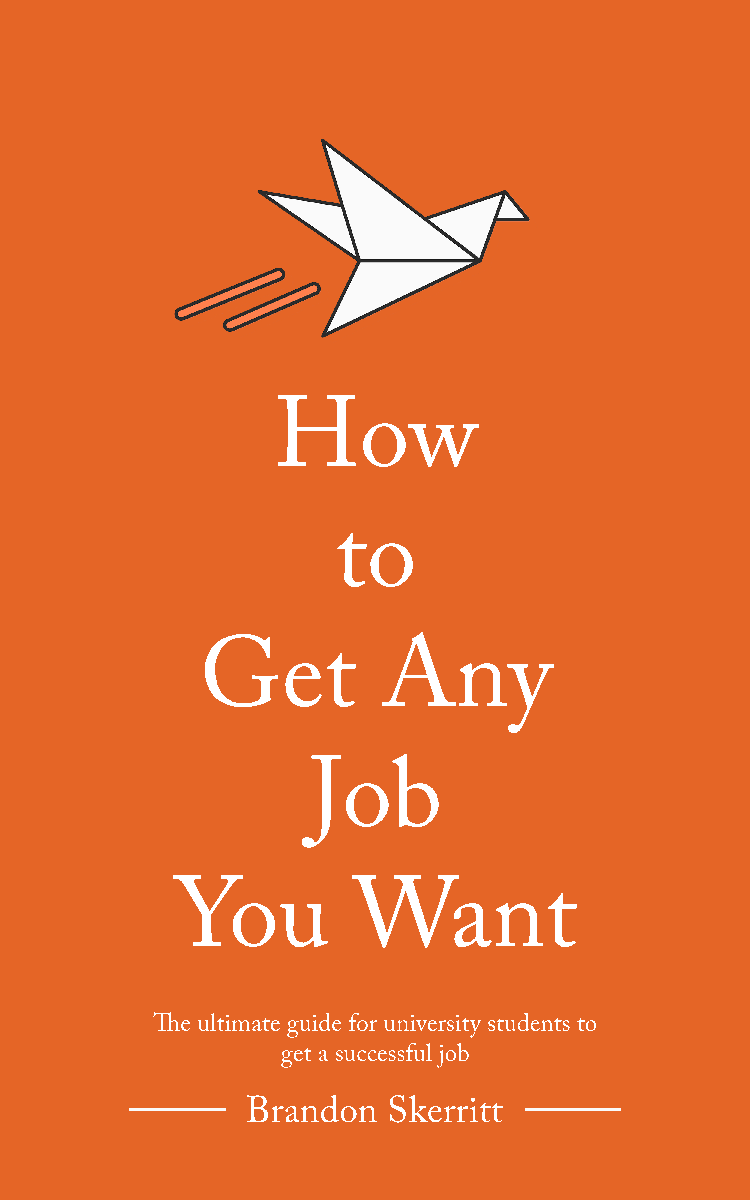
\includepdf{howtoget.pdf}


\begin{flushleft}
\clearpage
\pagenumbering{roman}
Dedicated to everyone who said I couldn't achieve great things, for
making me push that little bit harder every single day.
\end{flushleft}
\newpage
\section*{Acknowledgments}


The process of writing this book repeatedly made me wish I was dead. But
once I was done, I felt great. I was fortunate enough to have a group of
people who worked with me to bring this book to life.
\bigbreak
Hannah Blair, one of my mentors, is one of the most amazing people I've
met. I want to thank her for writing the best blogpost on Facebook I
could find, which I've used here. Her support since I've met her has
been invaluable
\bigbreak
Ibrahim for editing this book, making it the best book it could possibly
be. Many, many thanks Ibrahim.
\bigbreak
Olivia, for supporting me throughout all of this and for always
believing in me.
\bigbreak
Ciaron, for many good memories on the high seas and being an overall
good friend.
\bigbreak
Katie for reading the book and supporting me. I couldn't have done it
without your support!
\bigbreak
Many thanks to all who contributed on GitHub. Janogarcia for the
chaptering issue.

\newpage
\section*{Copyright}
Copyright © 2018 by SeventyTwo Publishing Limited on behalf of Brandon
Skerritt

All rights reserved. This book or any portion thereof

may not be reproduced or used in any manner whatsoever

without the express written permission of the publisher

except for the use of brief quotations in a book review.

Printed in the United Kingdom

First Printing, 2019

Published by SeventyTwo Publishing Limited.

ISBN 978-1-9160463-1-3

www.skerritt.blog
\newpage
\newpage
\tableofcontents
\newpage
\pagenumbering{arabic}
\setcounter{page}{1}
\section{Preface}
Professional skills, Just the mere murmur of the word makes me want to
fall asleep. It's such a boring topic, there's no getting around that.
So many people fall asleep in professional skills classes or never take
the time to learn these vital skills.

This makes a large difference between the people who took the boring
class and the people who didn't. So many people apply for graduate jobs
every single year, I'm willing to bet around 95\% of them have no
experience with professional skills. Because of this, there is a gap in
the market. If you have even basic professional skills, you're going to
look better than the 95\% of the candidates that have applied.

Professional skills are vital. Even if you do not wish to learn much
about it. To the nerds out there, like me, who have studied professional
skills we know this to be true. It is a boring subject, but if you study
this boring subject, you're going to look like the best thing since
sliced bread to employers.

Degrees don't matter. Unless you don't have one. If you have one, it
doesn't matter. 99\% of the people applying for graduate junior
positions have degrees. A degree will not make you stand out, no matter
how hard you work towards that degree. You need to differentiate
yourself, by showing that you are more than just a degree title. One of
the ways you could do this is by learning professional skills.

This book is written for everyone who understands that this is a vital
skill but does not have the knowledge or means to study it. This book is
written for everyone who desperately wants to learn these skills but
falls asleep in the lectures on them.

If you have no interest in getting an increase in salary before you
start, or no interest in being the best intern a company has ever had,
then put this book down. Do not read it. This is not for you.

One of the people who read the original draft on this got a promotion
before they started. Their CV was "the best thing we had ever seen"
and because of this, the person was deemed a god amongst everyone who
didn't have basic knowledge of constructing a CV.

Let me tell you a secret. For a select few who are obsessed with
professional skills, getting internships is a game. I am not joking. One
of my friends got 36 internships in his first year at the likes of Bank
of America, Barclays, Royal Bank of Scotland, Amazon, Apple, and many
more. I have more friends who have achieved similar feats.

For a select few, professional skills are a game. I've interviewed as
many of them as I could to learn the secrets to the game, how to get any
job you want. This book is a compilation of wisdom from that exclusive
group and much more.
\subsection{Career vs Job}
Let's get right into the business of the day. A job is something you do
for money. Your part time Tesco work is a job. A career is what your
life is, what you're doing with your life. This is anything that can
take over your life. A professor at University, for example.

With a job, you work a shift and that's it. You don't do anything else.

With a career, you work a shift, you go home, and you work some more.
You may go to conferences, you may network, you may learn some things in
order to improve yourself at your job. Here are the biggest differences:

\begin{center}

\begin{tabular}{||c|c||}
 \hline
 Career & Job \\ [0.5ex] 
 \hline\hline
 Long term & Short Term \\ 
 \hline
 Lots of growth and opportunities & Low or no growth \\
 \hline
Earning experience & Earning money \\
 \hline
Go above and beyond & Doing the bare minimum \\
 \hline
Happy that you get to work & Angry or frustrated that you're forced to
work \\ 
\hline
Aligned with the core values of the company & Uninterested or doesn't
care about the core values \\
\hline
Looking to move up the corporate ladder & Looking for a new job that
pays more \\
\hline
A career is a journey & A job is a grind \\
[1ex] 
 \hline
\end{tabular}
\end{center}

\subsection{The Job Cycle}
When you're in university, there's a certain cycle you normally have to
follow in order to get a good graduate job. The cycle is:

$$\hbox{Insight days} \rightarrow \hbox{Spring internships} \rightarrow \hbox{Summer internships} \rightarrow \hbox{Placement year} \rightarrow \hbox{Graduate job}$$

You don't need to do all of these things. The typical way most people go
around it is:

$$\hbox{Summer internships (or a placement year)} \rightarrow \hbox{Graduate job}$$

The lower you start on this cycle, the more likely you are to get a job.
This cycle doesn't matter that much, unless you're applying somewhere
exclusive. If you want to work somewhere like Bank of America, you'll
need to follow this cycle.

Bank of America would rather hire someone who went through the whole
cycle with them than someone who didn't. It matters here, since they are
such a big company even their insight days fill out quickly. They don't
need to bother with people who have only done an internship, if they
have hundreds who have done insight days or are even campus ambassadors
for them.

The lower levels (insight days, spring internships, sometimes summer
internships) carry over from other companies in the same industry.

If you did insight days and a spring internship at BlackRock, Bank of
America will think that's really good as you're in the industry. Of
course, they'll always pick someone who has worked for their company
over someone who's just worked at a competitor, but you can't expect to
do 20 insight days / 20 spring internships just to get a chance at a
company.

Most insight days / spring internships are just advertisements for a
company.
\subsection{Landing That Job}
It's better to blanket apply to as many companies as possible. And when you get an interview, focus intently on winning. Ideally, we'd want to apply to 100 companies with absolute precision, instead of the shotgun approach. But that's simply not possible.

If you have an internship, here's some good advice from a recruiter on
how to turn that internship into a graduate job.

This advice comes from Andrew Osayemi.

\begin{quote}
So, you are fortunate to have a spring or summer internship \& are
looking for 1 piece of unconventional advice, to help increase your
chances of being offered a full-time graduate job?

Well the advice is very simple. Ask everyone on your team if they
would like a tea or coffee every 2--3 hours each day
Do it with a warm smile.

If they say no still smile \& politely say "no problem, please let
me know if you need anything!"

And if they say yes, write down their order carefully so you don't mess
it up including any special requests (soya milk, 10 sugars etc)
When you return with their beverage of choice, again make sure you give
it to them with a warm smile

Now the next 10 seconds is crucial

You have an opening to ask how their day is going, if they have any work
for you to do, if you can book a convenient time to work shadow them,
did they watch the latest reality show etc.

Very soon your likeability factor will be increased which greatly
impacts your chances of being offered a full-time graduate offer!

I've given this advice to countless students whom I have coached via
Rare Recruitment \& the feedback is It works!
\end{quote}

As a small note, this actually depends on what you want to do. If you
want to work for the big 4 of tech, working really hard for those 4 make
sense. But there's another approach if you just want to get any job in
your field.

The approach is simple. You fire off as many CVs as possible to as many
companies as possible. While in this book, I'm under the assumption you
want a specific job at a specific company, this approach also works.

Ideally, you want to be able to perform intensive research on every
company. You want to customise everything for each company. You also
want to apply to as many as people while maintaining this work load.
Sadly, this isn't possible to achieve. Think of this as a dial between
two extremes. On the one extreme, you have the shotgun approach. Apply
to every single company you can without prior research or customisation.

On the other extreme, you have the sniper approach. You pick 3 or 4
companies and go in hard.

What you want to decide is where you sit on this dial. Where do you want
to sit between these two extremes? Here are some examples that will help
you, whichever one you choose:

\begin{itemize}
\item
  Shotgun apply to 100s of companies. The companies that really interest
  you, try the sniper approach.
\item
  Pick 20 or 30 companies to apply to and learn about them in depth. 
\end{itemize}
At the end of the day, the company doesn't care about you. Why should
you spend hours and hours researching a company that doesn't care? Maybe
you really want to work for that company. Don't read this book and think
"huh, this approach will work for me". Decide for yourself what will
and won't work.

\subsection{Your University's Careers Team}
Your university's careers team is an elite squad of experts whose entire
jobs are to get you great jobs. This book isn't meant to be a
replacement for them, it goes hand in hand with them. They can interview
you, look at your CV \& more to help you get prepared.

You can find out how to access your university's careers team by
Googling "[University name] careers team".
\subsubsection{My University's Careers Team Is Bad}
It happens. The good news is that you're already on your way to becoming
an expert in employability skills. By reaching out and reading this
book, you're already doing 90\% more than anyone else applying for that
job - learning more about employability skills.

For practice with interviews - go to as many as possible. Apply to
companies you'll likely never work at just to get interview experience.
The more you do, the better. When you're at an interview, make friends
with the other candidates and work together to achieve greatness. To get
great jobs. They'll likely be able to help you with your CV \& other
things.
\subsection{One Last Thing}
This book isn't a one size fits all book. The recruitment industry is
large. So large in fact, that it's impossible to cover every single
titbit. In some industries, a nicely designed CV is essential. In
others, anything other than black and white is seen as a monstrosity.
While I try my best in this book to guide you along this path, know that
you need to research yourself. I can't possibly cover every single
industry here.
\newpage
\section{Curriculum Vitae}
A Curriculum Vitae (CV) or a resume is one of the most vital parts of
job hunting. Put simply, it is a piece of paper you give to a recruiter.
This recruiter decides if you are worth the time to interview based on
this bit of paper.

Every job requires a CV. Sometimes, the job will force you to rewrite
your entire CV on their website. Even if it does, you'll still need a
CV.

As such, writing a good CV is the key to getting a good job.

The CV is a summary of your professional life so far. It features your
education, your work experience, skills and more.

Most times a person reads the CV, but sometimes machines can also read
it. Recently artificial intelligence is being used to read CVs. When a
human reads your CV, they don't exactly read it. Estimations say that
they spend 7 seconds on your CV, but this isn't true. If you were in the
position of looking at CVs and you saw something that looked spiritless,
would you bother reading it? I know you wouldn't. That's why your CV
needs to catch their eyes. It needs to make them curious and interested
in you within the first second or two. First impressions matter here, A
lot.
\subsection{Personalising Your CV}
Your CV will impress the person reading it if it's customised to them.
Everyone likes a customised birthday cake more than a regular Tesco own
brand birthday cake.

Make it look like you're perfect for the job because the employer only
wants the perfect candidate. The thing with applying for a very large
organisations is that they have no shortage of candidates. Why settle on
someone mediocre when 2 weeks later you'll have someone perfect for the
role? You need to act perfect and believe you are perfect for the role.

\subsubsection{Keywords Is the Keyword of This Section}
An AI looks for keywords. They do not have an average time of looking at
your CV.

A recruiter will insert a bunch of keywords into a computer program. The
program will scan each CV and give the CV a score on how many keywords
the CV has. This is why it is important to know what keywords to put
into your CV. But, having an A4 piece of paper with font size 2 to fill
it to the brim of keywords might not work. You don't know whether they
will use a human or a machine - or even both. Machines can rank your CV
depending on how `clean' it is too.

To insert keywords, you need to know what job you are applying for and
what company.

Let's say you apply to Barclays for a summer analyst position.
First you would Google around. Search for terms like "Barclays CV
keywords" and "Summer analyst keywords CV". If these do not return
anything then read the description.

A part of the description in 2018 states this:

\begin{quote}We are looking for bright, personable individuals who have the ambition to succeed and an impetus to learn and make the most of this
fantastic opportunity within a competitive environment.
\end{quote}

Barclays are looking for people who love learning. Who want to make a
difference to themselves and to the world and are above all, kind.

You should customise your CV to show that you love learning. You are
kind hearted (volunteering work can prove this, for example) and
understand that it is a competitive position. Try to use the keywords
themselves. Barclays say you need "an impetus to learn", you can write
in your CV profile that you have an impetus to learn. You should show
that you need this position.

To customise your CV, analyse the job description. Obsessively read it
and highlight keywords that come up. They say that they want someone
with strong self-motivation? Find something you've done that proves this
and put it on to your CV. Just like with the Barclays example earlier,
it's all about matching your CV up to the job description as much as
possible.

By inserting keywords into the CV you'll be able to pass the keyword
test performed by machines, as discussed earlier. But please do not puke
keywords onto your CV, it has to look natural.

Read the job description, the responsibilities, the specific
requirements, the location. If you see a word you don't know, Google it.
That word you don't know is likely a keyword. Remember the Barclays
example from earlier? It's like they've grabbed a thesaurus and randomly
inserted words into the job description. These words are keywords.

Some keywords come up and up again in many jobs such as:

\begin{itemize}
    \item Teamwork
    \item Time management
    \item Microsoft Office
    \item Leadership skills
    \item Computer literacy
\end{itemize}

Let's say a job description has this sentence in it:
\begin{quote}
    Required: Advance knowledge of Microsoft Applications (Word, Excel, PowerPoint
\end{quote}

Then instead of writing "Microsoft Office" on your CV you write:

\begin{quote}
    Advance knowledge of Microsoft Software (Word, Excel, PowerPoint)
\end{quote}

If the machine reads your CV, you'll pass the keyword test. If a human
reads your CV, they may not remember the job description exactly, which
is good. When they read "Advance knowledge of Microsoft Software\ldots"
something will click in their head which makes you stand out. That
something is that their subconscious memory recalls the keywords used in
the job description.
\subsubsection{Making the CV Fit Around You, Not You Trying to Fit into a CV Template}
If you're applying for a job that requires programming, have a
languages section on your CV that talks about all the languages you
know. Or if you know other languages, include them. There isn't a one
size fits all CV that's perfect for you. You need to make the perfect CV
for you.

It's also best to rate your skills. If you're fluent in German, say
you're fluent. If you're not fluent but still quite good, write
intermediate. Be honest, don't lie that you're fluent in Mandarin as the
job might need that you are.

Most people fire off blankets of CV's to every single recruiter on their
LinkedIn or job recruiters like it's the last thing you'll ever do. Do
not do this. Customisation per job is vital.

\subsubsection{Lie about your Location}
Want to get a job in London? Then write "London" on your CV.

This won't work well if you write "London" and you live in Scotland
unless you plan to move.

If you get called up on it say you're going to relocate, or you enjoy
commuting.

You need the employer to think that if they hire you, they won't come
into any problems like you living an hour away.
\subsubsection{How to Research an Organisation}
You need to know about an organisation before you apply for a job there.
You can't apply to an organisation you know nothing about and expect to
get the job. In order to be the perfect candidate, you need to be an
expert on this organisation.

Some of the things you want to find out are:

\begin{itemize}
\item
  The mission statement of the company
\item
  Who founded it and why
\item
  A brief history of the company
\item
  Current CEO of company
\item
  Where they are based
\item
  Products and services
\item
  Competitors
\item
  Current issues
\item
  Current news
\item
  Ethics \& morals
\item
  Culture
\item
  The people you will be working with / the person interviewing you
\item
  Career development
\item
  Travel opportunities
\end{itemize}

Once you've researched about them, add the things you've found to a word
document and print it out. Go over this document on the way to the
interview. You do not need to memorise every company you apply for. Use
this information in your cover letter and learn the information the day
before your interview.

You could Google most of these. Just Google "[Companies name] [thing you want to find out]". When you research a company, the best website you should concentrate on is the company's own website. For history, you should look at the company's Wikipedia page. For current
news, you can Google search the company and click the "news" tab.

For most companies, Bloomberg contains a "snapshot" of the company.
This includes the key executives for the company, their age, their
annual compensation, a company overview, how many employees they have
and more. The key thing about these snapshots are the ""key developments" section whereby Bloomberg lists the most important news
and developments for a company.

To find a Bloomberg snapshot of a company, Google "[company name] Bloomberg snapshot".

If the company is especially big, chances are that the Economist has
written an article about them at some point. Find sources you like \&
trust, and search to see if that company has come up in these sources.


\subsection{Writing a CV}
Now we know about customising a CV, let's get into how to write a CV.
The first most important rule is that your CV should be 1 page. Not
double sided but one page. If you have 15+ years of experience then 2
pages is okay, but 1 page is always preferable.
\subsubsection{Choosing the Right CV Template}
Choosing the right CV template is always important. You could try to
create your own template, but I don't suggest you do this unless you're
good at design. The simplest and easiest way to find a good template is
to Google "CV Template" and pick one you like.

Make sure the template is well designed and it has to be visually
appealing. The template should be slightly sparse of information. A CV
with little information on it looks more appealing than a CV full of
information. The recruiter is used to CVs with paragraphs upon
paragraphs of information. If you have little information, it will catch
their eye. Try not to disclude stuff that's directly relevant to the
position, you want to be the best person for the job.

If you know a little tiny bit about computers, you can Google "LaTeX CV
templates" to get some nice templates for free. If it's on Overleaf or
ShareLaTeX then it's easier to use. LaTeX is like a programming language
but for writing.

A well-designed CV is more important than most people think. Well
designed does not have to equal "pretty colours and nice shapes".

In some industries, a well designed CV is a burden. Employers can hate
them with a burning rage. The recruitment industry is less "this one
tip works for everyone" and more "this one tip is really cool for a
specific part of the industry". Well designed CVs may be appreciated at
tech start-ups or design companies, but at other places like law firms
they can be hated. While in this book I advocate for colour CVs, know
that you need to perform your own research and find out if its
appropriate for your industry.

Another downside to using well designed CVs is that Applicant Tracking
Software can't read them. This is the software / AI used to determine
whether or not you are the right candidate.

Instead of reading these chapters and thinking "this is perfect for my
industry" I implore you to think "this is a good idea, but I wonder if
my industry likes this?"

If you believe the answer to be "yes, my industry likes this" then go
ahead.

But, the benefits for well designed CVs still exist. No one else will
have a CV like yours, so you'll stand out. Also, you can have a well
designed CV and have a plain black / white layout. Whitespace is your
friend here. Lots of space, sparse information.

You have to decide for yourself what is good and what is bad. All
industries are different.

My friend Chris has so many internships he's lost count. These include
places like Bank of America, Google, Facebook and many, many more. His
CV is black \& white and it worked pretty well for him. Try to find
people in the industry you're applying for like Chris who have a lot of
experience applying to jobs. Ask them what the industry is like. You can
use LinkedIn for this.

Your CV needs to be eye-catching, it needs to be designed well. It needs
to look good and have the correct information in it.

Personally speaking, I use NovoResume.com for all of my CV needs. I have
been using them for years, and they've never once let me down.

Your university careers team might also have templates for you to use,
but I would recommend at least modifying this template. Thousands of
people will use your universities careers template every year, try to
make it unique and make it your CV. If you've found 2 or more templates
you really like, and you don't know which one to use, just ask your
university careers team.

If your CV is visually stunning, the employer will love it. They read so
many of the same black \& white PDF documents filled with information
every day they're desperate to find something that has a hint of graphic
design.

Another thing to note is the use of progress bars as indicators of how
well you know something. Saying you're 4/5 for speaking Spanish, what
does that mean? You're not natively fluent in it, but you know some of
it.

Especially on things that constantly change. Say you graded your CSS
knowledge 75\% (it's a programming language). CSS then gets a huge
update. Do you now know 50\% of CSS?

Going hand in hand with a well-designed CV, don't crinkle your CV or put
folds in it if you print it out. It has to look like it just came out of
a printer. Never, ever hand over a CV with a crinkle or fold in it.
\subsubsection{Achievements \& Jobs on a CV}
When writing out your CV, list your achievements at a job. Don't list
the duties you had to do. Everyone has to do stuff at a job,
achievements are more impressive. Make sure the CV is visually appealing
and sparse of information. You want to tell a story in as few words as
possible. Put your jobs in reverse-chronological order so your most
recent work appears at the top of the CV.

If I was to say that I was the best Student Union officer that would
make me sound big headed. If I was to change that to "changed Student
Union approval rating from 30\% to 90\%" it would sound even more
impressive and not so egotistical.

Achievements are important too. Try to make your achievements in this
format:
\begin{quote}
    I did X by doing Y as proved by Q
\end{quote}

As a general rule you need to have some sort of statistic related to the
achievement. It makes the achievement sound so much more impressive.
Mixing this achievement rule with statistics will go a long way for you.

Don't include jobs if it's not relevant. If you're applying to be an
investment banker and you worked at an ice cream shop for a week, it's
not really helpful for you to put that on. It'll just make your CV look
messy. If you have no experience, it will be more helpful to put your
education on it. You want to balance your education and work experience.
If you've never worked anywhere relevant before, you'll want to include
your A-levels and university modules with grades. If you've worked in
industry, as an internship or whatnot then you might not want to include
A-levels in order to write more about this experience.

Real world experience is always worth more than education, so try to
disclude as much information of your education as possible. But make
sure to put university on there. Don't include primary / secondary
school. The earliest you can go back to is A levels.

If you're applying for a job in academia, your education matters a lot
more than normal. If you have a perfect mix of work experience and
education, try to list your education shortly. Only include the modules
that are relevant to the job. If you're applying for a job in game
design and you've done modules on game design, include them.

The single most important thing you can do to make your CV stand out is
to customise your CV per job.

\subsubsection{How to Spell-Check Your CV}
You need to avoid spelling and grammar mistakes at all costs. It is the
difference between you getting a job and you not getting the job. The
simplest form of spell checking you can do is to run the Microsoft Word
spell checker. But, this isn't good enough. You actually need to read
your CV, and then get someone else to read it for you.

Your university's careers team is perfect for this. Almost every careers
team will have some form of session or drop in clinic for them to read
your CV and pick up on anything that's wrong. When in doubt, visit your
careers team.

Instead of Microsoft Word's spell checker, I use Grammarly.

\subsubsection{To PDF or Not to PDF}
Always send your CV as a PDF unless they absolutely specify it has to be
sent in a format they require.

The PDF is designed to be readable on any machine. The way the PDF looks
on your machine is the exact same way it'll look on any other machine.
Anyone can open a PDF. PDFs are supported in Internet Explorer or
Chrome. With Microsoft Word, if they have a different Word version to
you it may look different. It may actually look worse to them than it
does to you. Also, not everyone has Microsoft Word; but everyone has a
web browser like Firefox or Chrome.

If they need the CV in plaintext (copy and paste) you have to change the
formatting. You can make sections using " --- ---". Like so:
\begin{quote}
Achievements\\
-\/-\/-\/-\/-\/-\/-\/-\/-\/-\/-\/-\/-\/-\/-\/-\/-\/-\/-

* Changed Student Union approval rating from 30\% to 90\%
\end{quote}
You can use an asterisk as a bullet point, as seen above.

\subsubsection{References}
No references available on request. No one I know that gets jobs does
this. Make it as easy as possible for the recruiter. Contacting you to
ask for references is another step to them, which makes it harder. Cut
out the middleman and put the contact details for your reference on the
CV itself.

I know that some references will write you letters, and that's good. You
should hand these in when they ask for qualifications (if they do) or
letters of recommendation. Please do not copy and paste your references'
letters onto your CV or attach them to the other blank side. It's just
not good.

You'll usually want 2 references, 1 academic and 1 work related. If you
have never worked somewhere before, use another academic reference if
you can or someone you have volunteered with. Or the head of a society
you're active in.

When you put the reference on your CV, it should look like this:\\
Name\\
How they know you (ex-boss, ex-co-worker)\\
Contact details (email, phone)

That's it. No "I went drinking with him every Friday". No stories or
anything, short and sweet.

Make sure you ask the person if you can use them as a reference. Make
sure they will only say good things about you. If they want to "be
honest" about you, find someone else. Your references should gleam at
the opportunity to talk about how amazing you are.

In a warm Starbucks once I was talking to a recruiter. They talked about
how many people put references down without making sure the referencer
is okay with it. Or they'll put a reference down that isn't too keen on
the person. The recruiter would often call these references and get:

\begin{quote}
\emph{"They were alright, they did the job"}
\end{quote}

or even worse:

\begin{quote}
\emph{"Who are they again?"}
\end{quote}

It's important to make sure your references know you and love you. Be
very careful with what information you put down too.

If you put down the references personal phone number and your CV gets
shared around, you've shared personal information with people the
reference doesn't even know about. This is violating many Data
Protection Act Regulations.

In some countries, you don't even need to put references down on your
CV. References are sometimes the very last thing a recruiter asks for.
You could instead use that reference space for something more important.

Like with choosing a well designed CV or a plain CV, you need to decide
for yourself. While in the UK it is traditional to put references down,
you need to consider the benefits and downsides of it.

\textbf{Benefits}

\begin{itemize}
\item
  Easy for the recruiter to find out more about you. Easier for the
  recruiter is always better
\end{itemize}

\textbf{Downsides}

\begin{itemize}
\item
  Takes up precious space on a CV. CVs are supposed to only be 1 page
  long, you could use that space for something else.
\item
  Not needed in most countries.
\item
  You could accidentally violate Data Protection Regulations.
\end{itemize}

\subsubsection{Make It as Easy for Your Employer as Possible}
Referencing what I said earlier, make it as easy for your employer as
possible. Think about who you are applying to. If you're applying in the
tech industry, chances are that they are reading your CV on a computer,
so hyperlinks in CVs are cool. If not, don't include them as they don't
look good when printed out.

Are you applying to be a graphic designer? The design of your CV matters
the most. Are you applying to be a game developer? You could make your
CV as a game, like Robbie Leonardi did here:
\href{http://www.rleonardi.com/interactive-resume/}{{www.rleonardi.com/interactive-resume/}}

Really think about who you are applying for and how you can make your CV
better for them.
\subsubsection{Have a "Profile" Section}
This profile is a small section of your CV that includes a brief summary
of your skills, experiences and goals. It is your elevator pitch.
Imagine you are in an elevator with the recruiter of a large company.
You have 30 seconds to convince them to care about you enough to want to
interview you. This is the elevator pitch. A good profile makes people
interested in you. It gives them a reason to read on and pay attention
to your CV.

This is truly customised to you. I really cannot tell you what to write.
Your elevator pitch should talk about who you are, what you do, your
education, and your goals in life. A good profile will break these
rules. It's one thing to follow the rules, but in order to stand out you
need to break these rules. My profile is:
\begin{quote}
"Obsessive learner and problem solver, always looking for the next big problem to solve"
\end{quote}

Your elevator pitch talks about your education \& experience, your CV
profile talks about you as a person. If they want to know about your
education \& experience, they'll simply read on. Your principles and
goals in life are discovered, not invented.

My friend's profile says:

\begin{quote}
\emph{"I love what I do -- turning ideas into reality by coding. "}
\end{quote}

It's incredibly hard for me to describe this, since it has to be
personalised to you. No one can tell you what to write here, but keep in
mind that you'll discover what you love if you keep it in the back of
your head for long enough.

\subsubsection{Bullet Points, Paragraphs \& Action Verbs}
Bullet Points. Always try to have bullet points. You're allowed to
include paragraphs, but if everything in your CV is a paragraph it'll
look extremely dull. Bullet points are more readable.

Personally speaking, the only time I use paragraphs is for my
achievements, when I want to tell a story. Everything else is bullet
points. You should use action verbs in your bullet points to make it
sound powerful. Instead of saying:
\begin{quote}
\emph{"I led a project"}
\end{quote}

You can say:

\begin{quote}
\emph{"I orchestrated a project"}
\end{quote}
Here is a list of 185+ action verbs you can use, from the website The
Muse\footnote{\href{https://www.themuse.com/advice/185-powerful-verbs-that-will-make-your-resume-awesome}{{https://www.themuse.com/advice/185-powerful-verbs-that-will-make-your-resume-awesome}}
  accessed at 07/08/2018.}
  
\begin{longtable}}
\toprule
\endhead
\begin{minipage}[t]{0.47\columnwidth}\raggedright
\hypertarget{you-increased-efficiency-sales-revenue-or-customer-satisfaction}{%
\paragraph{You increased efficiency, sales, revenue, or customer
satisfaction}\label{you-increased-efficiency-sales-revenue-or-customer-satisfaction}}

\begin{itemize}
\item
  Accelerated
\item
  Achieved
\item
  Advanced
\item
  Amplified
\item
  Boosted
\item
  Capitalized
\item
  Delivered
\item
  Enhanced
\item
  Expanded
\item
  Expedited
\item
  Furthered
\item
  Gained
\item
  Generated
\item
  Improved
\item
  Lifted
\item
  Maximized
\item
  Outpaced
\item
  Stimulated
\item
  Sustained
\end{itemize}\strut
\end{minipage} & \begin{minipage}[t]{0.47\columnwidth}\raggedright
\hypertarget{you-thought-of-and-brought-a-project-to-life}{%
\paragraph{You thought of and brought a project to
life}\label{you-thought-of-and-brought-a-project-to-life}}

\begin{itemize}
\item
  Administered
\item
  Built
\item
  Charted
\item
  Created
\item
  Designed
\item
  Developed
\item
  Devised
\item
  Founded
\item
  Engineered
\item
  Established
\item
  Formalized
\item
  Formed
\item
  Formulated
\item
  Implemented
\item
  Incorporated
\item
  Initiated
\item
  Instituted
\item
  Introduced
\item
  Launched
\item
  Pioneered
\item
  Spearheaded
\end{itemize}\strut
\end{minipage}\tabularnewline
\bottomrule
\end{longtable}

\begin{longtable}}
\toprule
\endhead
\begin{minipage}[t]{0.47\columnwidth}\raggedright
\hypertarget{you-saved-the-company-time-and-money}{%
\paragraph{You saved the company time and
money}\label{you-saved-the-company-time-and-money}}

\begin{itemize}
\item
  Conserved
\item
  Consolidated
\item
  Decreased
\item
  Deducted
\item
  Diagnosed
\item
  Lessened
\item
  Reconciled
\item
  Reduced
\item
  Yielded
\end{itemize}\strut
\end{minipage} & \begin{minipage}[t]{0.47\columnwidth}\raggedright
\hypertarget{you-were-in-charge-of-a-project}{%
\paragraph{You were in charge of a
project}\label{you-were-in-charge-of-a-project}}

\begin{itemize}
\item
  Chaired
\item
  Controlled
\item
  Coordinated
\item
  Executed
\item
  Headed
\item
  Operated
\item
  Orchestrated
\item
  Organized
\item
  Oversaw
\item
  Planned
\item
  Produced
\item
  Programmed
\end{itemize}\strut
\end{minipage}\tabularnewline
&\tabularnewline
\begin{minipage}[t]{0.47\columnwidth}\raggedright
\hypertarget{you-manage-a-team}{%
\paragraph{You manage a team}\label{you-manage-a-team}}

\begin{itemize}
\item
  Aligned
\item
  Cultivated
\item
  Directed
\item
  Enabled
\item
  Facilitated
\item
  Fostered
\item
  Guided
\item
  Hired
\item
  Inspired
\item
  Mentored
\item
  Mobilized
\item
  Motivated
\item
  Recruited
\item
  Regulated
\item
  Shaped
\item
  Supervised
\item
  Taught
\item
  Trained
\item
  Unified
\item
  United
\end{itemize}\strut
\end{minipage} & \begin{minipage}[t]{0.47\columnwidth}\raggedright
\hypertarget{you-changed-or-improved-something}{%
\paragraph{You changed or improved
something}\label{you-changed-or-improved-something}}

\begin{itemize}
\item
  Centralized
\item
  Clarified
\item
  Converted
\item
  Customized
\item
  Influenced
\item
  Integrated
\item
  Merged
\item
  Modified
\item
  Overhauled
\item
  Redesigned
\item
  Refined
\item
  Refocused
\item
  Rehabilitated
\item
  Remodelled
\item
  Reorganized
\item
  Replaced
\item
  Restructured
\item
  Revamped
\item
  Revitalized
\item
  Simplified
\item
  Standardized
\item
  Streamlined
\item
  Strengthened
\item
  Updated
\item
  Upgraded
\item
  Transformed
\end{itemize}\strut
\end{minipage}\tabularnewline
\begin{minipage}[t]{0.47\columnwidth}\raggedright
\hypertarget{you-changed-or-improved-something-1}{%
\paragraph{You changed or improved
something}\label{you-changed-or-improved-something-1}}

\begin{itemize}
\item
  Centralized
\item
  Clarified
\item
  Converted
\item
  Customized
\item
  Influenced
\item
  Integrated
\item
  Merged
\item
  Modified
\item
  Overhauled
\item
  Redesigned
\item
  Refined
\item
  Refocused
\item
  Rehabilitated
\item
  Remodelled
\item
  Reorganized
\item
  Replaced
\item
  Restructured
\item
  Revamped
\item
  Revitalized
\item
  Simplified
\item
  Standardized
\item
  Streamlined
\item
  Strengthened
\item
  Updated
\item
  Upgraded
\item
  Transformed
\end{itemize}\strut
\end{minipage} & \begin{minipage}[t]{0.47\columnwidth}\raggedright
\hypertarget{you-wrote-or-communicated}{%
\paragraph{You wrote or communicated }\label{you-wrote-or-communicated}}

\begin{itemize}
\item
  Authored
\item
  Briefed
\item
  Campaigned
\item
  Co-authored
\item
  Composed
\item
  Conveyed
\item
  Convinced
\item
  Corresponded
\item
  Counselled
\item
  Critiqued
\item
  Defined
\item
  Documented
\item
  Edited
\item
  Illustrated
\item
  Lobbied
\item
  Persuaded
\item
  Promoted
\item
  Publicized
\item
  Reviewed
\end{itemize}\strut
\end{minipage}\tabularnewline
\begin{minipage}[t]{0.47\columnwidth}\raggedright
\hypertarget{you-supported-customers}{%
\paragraph{You supported customers}\label{you-supported-customers}}

\begin{itemize}
\item
  Advised
\item
  Advocated
\item
  Arbitrated
\item
  Coached
\item
  Consulted
\item
  Educated
\item
  Fielded
\item
  Informed
\item
  Resolved
\end{itemize}\strut
\end{minipage} & \begin{minipage}[t]{0.47\columnwidth}\raggedright
\hypertarget{you-overview-or-regulated}{%
\paragraph{You overview or regulated}\label{you-overview-or-regulated}}

\begin{itemize}
\item
  Authorized
\item
  Blocked
\item
  Delegated
\item
  Dispatched
\item
  Enforced
\item
  Ensured
\item
  Inspected
\item
  Itemized
\item
  Monitored
\item
  Screened
\item
  Scrutinized
\item
  Verified
\end{itemize}\strut
\end{minipage}\tabularnewline
\begin{minipage}[t]{0.47\columnwidth}\raggedright
\hypertarget{you-achieved-something}{%
\paragraph{You achieved something}\label{you-achieved-something}}

\begin{itemize}
\item
  Attained
\item
  Awarded
\item
  Completed
\item
  Demonstrated
\item
  Earned
\item
  Exceeded
\item
  Outperformed
\item
  Reached
\item
  Showcased
\item
  Succeeded
\item
  Surpassed
\item
  Targeted
\end{itemize}\strut
\end{minipage} & \begin{minipage}[t]{0.47\columnwidth}\raggedright
\hypertarget{you-were-a-research-machine}{%
\paragraph{You were a research
machine}\label{you-were-a-research-machine}}

\begin{itemize}
\item
  Analysed
\item
  Assembled
\item
  Assessed
\item
  Audited
\item
  Calculated
\item
  Discovered
\item
  Evaluated
\item
  Examined
\item
  Explored
\item
  Forecasted
\item
  Identified
\item
  Interpreted
\item
  Investigated
\item
  Mapped
\item
  Measured
\item
  Qualified
\item
  Quantified
\item
  Surveyed
\item
  Tested
\item
  Tracked
\end{itemize}\strut
\end{minipage}\tabularnewline
\begin{minipage}[t]{0.47\columnwidth}\raggedright
\hypertarget{you-brought-in-partners-funding-or-resources}{%
\paragraph{You brought in partners, funding, or
resources}\label{you-brought-in-partners-funding-or-resources}}

\begin{itemize}
\item
  Acquired
\item
  Forged
\item
  Navigated
\item
  Negotiated
\item
  Partnered
\item
  Secured
\end{itemize}\strut
\end{minipage} & \begin{minipage}[t]{0.47\columnwidth}\raggedright
\strut
\end{minipage}\tabularnewline
\bottomrule
\end{longtable}

\subsubsection{Things to Include in a CV}
You have a template and you want to change a few things, here are some
things you might want to include:

\begin{itemize}
\item
  Personal details --- Telephone, professional email, location, name
\item
  Work experience
\item
  Achievements
\item
  Education
\item
  Hobbies and interests that relate to the job
\item
  Key skills relating to the job
\item
  Know any languages that relate to the job? Put them down!
\end{itemize}
You can also put a language down that doesn't relate to the job. If you
know an Asian language like Chinese and you put that into your CV, the
recruiter will instantly think you are some sort of super genius.

\subsubsection{What Not to Include in a CV}
\begin{itemize}
\item
  A head-shot / image of you. Unless the company specifies that they
  need this, do not do this. They do not want to see you.
\item
  Age and date of birth --- It's illegal for employers to ask about your
  age under the Equality Act of 2010.
\item
  Martial / Relationship status --- Again under the Equality Act of 2010
  they cannot ask this.
\item
  Every single thing you have ever done --- Make it short and customise
  it per job.
\end{itemize}
Let's just list all the things that the Equality Act of 2010 makes
illegal for employers to ask you:

\begin{itemize}
\item
  Marital status
\item
  Date of birth / age\footnote{Only if you must be a certain age for the
    job, such as selling alcohol.}
\item
  Gender
\item
  Dependants
\item
  General health\footnote{Unless it is required for the job E.G eye test
    for commercial driving.}
\item
  Religion
\item
  Disabilities\footnote{Only if there are requirements of the job that
    cannot be met with reasonable adjustments or the recruiter is asking
    to find out how to support you during the process. An employer is
    allowed to treat a disabled person more favourably than a non
    disabled person, so it may be best to put this down in some cases.
    Source:
    https://www.gov.uk/employer-preventing-discrimination/recruitment}
\item
  Spent criminal convictions
\item
  Trade Union membership
\item
  Ethnicity or other underrepresented characteristic\footnote{An
    employer is allowed to choose someone who is under-represented such
    as Women in Tech over someone who is not under-represented, so it
    may be best to put this down if it helps your application. Source:
    https://www.gov.uk/employer-preventing-discrimination/recruitment}
\item
  Pregnancies
\item
  Sexual Orientation
\end{itemize}
\subsection{Summary of This Chapter}
\subsubsection{Personalising a CV}

$\square$ Have you used a CV template?

$\square$ Have you customised the CV template to fit around you?

$\square$ Does your CV have keywords in it?

$\square$ Is your CV clean \& minimalistic?

$\square$ Do you have special sections related to the job? IE languages, skills,
achievements?

$\square$ Does your CV have contact details on it, and is the location where you
want to be / where you are?

$\square$ Do you have achievements at a job on your CV?

$\square$ Have you spell checked you CV?

$\square$ Is your CV a PDF?

$\square$ Do you have references, without "references available on request" on
your CV?

$\square$ Do you have a profile section?

$\square$ Do you have action verbs in your CV?

$\square$ Have you gotten rid of everything under the Equality Act of 2010, unless it benefits you in some way?
\subsubsection{Researching an Organisation}
Do you know these things about the company:

$\square$ Mission statement of the company

$\square$ Who founded it \& why

$\square$ A brief history of the company

$\square$ Current CEO of the company

$\square$ products \& services

$\square$ Competitors

$\square$ Current issues

$\square$ News

$\square$ Culture

$\square$ Career development
\newpage
\section{Cover Letters}
The cover letter is a letter that goes with a CV that explains why you
want a job. It can be the first chance you get to stand out to your
potential employer.

What makes a cover letter so difficult is that there is no clear-cut
formula to writing a cover letter.

Ultimately the goal of the cover letter is to draw attention to
yourself. It should be clear, concise and display competent language
skills.

It is important to note that not all jobs require a cover letter. It
should state it in the job description if it does require a cover
letter.
\subsection{Design of a Cover Letter}
Google "Cover letter templates" and find one you like. The exact same
advice from the CV applies here too. Make sure it's designed nicely. If
you use Novoresume, they also have cover letter templates.

\subsection{Length of the Cover Letter}
Some people write entire novels as cover letters, well, almost. Your
cover letter should be short. A full page at most.

The shorter a cover letter is, the better it will look. Don't try to
skimp on information to make it shorter. 4 paragraphs are around the
perfect length since it will follow a typical story arc.
\subsection{General Structure of a Cover Letter}
Start with an introduction. Make the reader aware of why you're writing
this. Include the job you're applying for. We'll go into each section
soon.

The 2nd paragraph is your skills, what you can provide to the company.

The 3rd paragraph should be why you want to work for the company.

The 4th paragraph is the conclusion. Mention that you look forward to
hearing back from them.

This follows a typical story arc. Start off with who you are, why they
should care, why you care about them, summarise and end.
\subsection{Some General Tips for the Cover Letter}
Don't talk about how great the position would be to you. Talk about what
you can bring the company, always have the company in mind. Show what
you're capable of within a cover letter. Try to tell a story. Stories
illuminate the human mind and intrigues them. Try to push them to read
more.

Do not make a one-size-fits-all cover letter. It's the same as the CV,
customise it per job. Job hunting is in itself a job.

As with a CV your cover letter may be keyword tested so try to include
some keywords that the employer wants to see.

Always send your cover letter as a PDF for the same reason you would
send a CV as a PDF.

Do not use weak or passive language. \href{http://www.hemingwayapp.com}{{http://www.hemingwayapp.com}} is an
online editor which will show you what is considered weak or passive.
Instead of writing "I feel", "I believe" write "I am confident that, "I
am positive that".

Try to limit the use of "I". This is a letter about how you meet the
employer's needs, not why it would be good to you.

The formality depends on the company. If you are applying for a tech
start-up formality likely isn't something they do. An old-fashioned
bank? Be as formal you can

\subsection{The Start of the Cover Letter}
A cover letter should have your information at the start:
\begin{itemize}
    \item First \& Last Name
    \item Street Address
    \item City
    \item Postcode
    \item Phone Number
    \item Email Address
\end{itemize}
Then comes your salutation. Dear Sir / Madam / Mrs / Mr / Ms / Dr. If
you know the person's name and their honorific, then you need to use
this. The letter should feel addressed to that individual person, it
should never feel like a blanket cover letter you've sent to everyone

\begin{quote}
John Gribbin

171 Fake street ct9 9lr

+0174857389

google@google.com"
\end{quote}
\subsection{First Paragraph}
The first paragraph is where you introduce yourself. What you're
applying for.

\begin{quote}"Dear Sir or Madam,

My name is Brandon Skerritt and I am applying for the position of
Bookseller at Waterstones, please find enclosed my CV."\end{quote}

In most cases they already know what your name is and what you're
applying for, so if you can don't include this part. Always include the
salutation. If you know the name of the person who will be reading this,
use their name.

As stated in How to Win Friends and Influence People:

\begin{quote}"Names are the sweetest and most important sound in any language."\end{quote}

Use keywords. Keywords and statistics are the secret key to unlocking
that first interview.

If you were referred to the job, mention that contact. Express
excitement that you've applied. The reader should feel like you would
die if you didn't get the job. That you want this job more than
anything.

\begin{quote}"I have the pleasure of being acquainted with one of the Counsellors on your staff, Eleanor Seville. She let me know about the open position and recommended that I contact you." \end{quote}

Recommendations are important. Some professionals state that they would
never have gotten the job if not for a recommendation.

The first paragraph should flow into who you are and why you want this
job. You can always say "I hope you are well" if you do not know what to
write.
\subsection{Second Paragraph}
The second paragraph is where you talk about your skills and experience.
Unlike a CV you do not use blunt bullet pointed language here but
instead talk about your experience, like a story. You can also explain
any gaps that might appear in a CV here.

Try not to regurgitate your CV in letter form. Think about what you're
writing and why you're writing it. Make it into a story. You need to
customise your cover letter per job, much like you'll customise your CV
per job.

This section should display that you have researched this position and
know what it is about and how your skills match with the position.

\begin{quote}"For as long as I can remember I've been an obsessive reader. I review books on GoodReads, I've written some fiction novellas in my spare time.
I've been a bookseller for the last 2 years at {[}Bookshop name here{]}
and have loved every second of it. As well as being a bookseller I've
trained new employees and managed the general every day running of the
store." \end{quote}

Sometimes people will use bullet points, it's entirely up to you. If
this was bullet pointed it would look like:

\begin{quote}"For as long as I can remember I've been an obsessive reader, having even written some fiction novellas in my spare time. I've been a bookseller for the last 2 years and in my role, I have achieved:

\begin{itemize}
\item
  Trained new employees although it wasn't my job
\item
  Broke the record for most amount of money earnt in made in a day.
  Previous record was £400, my team and I made £1200
\item
  Located a class photo book from the 1980s by calling up every store in
  the area to check for it. Just to make the customer happy."
\end{itemize}
\end{quote}

Bullet points make it shorter and easier to read but it also takes away
the humanity of a normal paragraph.
\subsection{Third Paragraph}
The third paragraph is why you're applying. What do you like about the
job or company you're applying to? Any nice anecdotes about the company?
After reading the last paragraph the recruiter should be curious. Why do
you want to change jobs if you love it? What's so special about this
company? \textbf{What can you do for the company?}

This is where you swing the bat and hit that ball out of the park. This
is where you show your determination and undying love for the company.
This is where the recruiter decides if you're different from the others.

\begin{quote}"Waterstones has always been my favourite bookstore. I've collectedover 11 stamp cards and try to go to Waterstones weekly to see what new books have been released. Sometimes I cannot help myself as a fellow book seller to rearrange books that have been misplaced or recommended books for your store based on the shelves. One such instance is a book titled "how to read water"; this book would have looked good next to The Cloud Collectors guide --- a book on reading clouds"\end{quote}
\subsection{Fourth Paragraph}
Fourth paragraph is the conclusion, where you wrap this all up.
Reiterate why you want to work there and display that you are happy that
you might have the opportunity to work there.

\begin{quote}"Your store is my favourite among the many Waterstones I have been to, and I've been to nearly all of them. I hope I have the opportunity to work at this fantastic store.

I look forward to hearing back from you,

Brandon Skerritt"\end{quote}

Another way to end this is:

\begin{quote}"Thank you for your time and consideration. I look forward to meeting with you to discuss my application further.

Yours sincerely,

Brandon Skerritt"\end{quote}
\subsection{Conclusion}
$\square$ Have you researched the company and you know what keywords to use?

$\square$ Have you discussed what you can bring the company, not what the
company can bring you?

$\square$ Have you customised it per job?

$\square$ Is your cover letter a PDF?

$\square$ Are you using active language (and not passive)?

$\square$ Does the formality of the cover letter match the formality of the job?
\newpage
\section{Personal Branding}
\begin{quote}"What are you doing?"

"I'm googling them" responded my friend with CVs strewn across her
table.

"This one's bad" she stated with authority. The CV itself looked good
enough for an interview but her research online showed she wasn't right
for the job.\end{quote}
One by one, she Googled them all. Education didn't matter, their
experience - for the most part, didn't matter.

Although this was a part-time waitressing job at a small local café,
their online portrayal mattered. It mattered so much that people with
amazing academical backgrounds and lots of experience were being tossed
to the side.

This is why personal branding is important. It is not only for the
entrepreneurs out there but for every single person. Most people believe
that personal branding doesn't affect them since they are not a
celebrity. The truth is, everyone has a personal brand. It's up to you
to decide when and how you'll take control of it. Your personal brand
exists, whether you like it or not.

A personal brand isn't makeup you're selling or being featured in
magazines. It is everything about your public life. Your Twitter,
Facebook, Instagram.

You do not have to be an entrepreneur to care about your personal brand.
When you apply for a job the recruiter will Google you. They'll want to
know:

\begin{itemize}
\item
  Does this person have a blog or website?
\item
  What does this person do in their spare time?
\item
  Any side projects?
  \item Is there anything bad about them online?
\end{itemize}

If you tick some of these boxes, you'll stand out from the rest.

There is often a quote given out in running circles:

\begin{quote}"It's okay to run slowly. You're still running laps around the people sitting on the sofa." \end{quote}

The same can be said for a personal brand. It's okay if your personal
brand doesn't have years of posts or tweets. It's okay if you only
started today. You're still doing better than those who have not
started.

Your personal brand will bring you more riches in life than any job you
could have. When we work somewhere, we say that thing is us. "I am a
lawyer" instead of "I practice law". "I am a programmer" instead of "I
program at work".

This way of thinking consumes your life. Your entire life rotates around
this one job, this one title.

This should not be the case. If you quit or you lose your job, then your
title goes away. If your title goes away, your entire life crumbles.

If you developed a personal brand and have friends and fans, then they
will continue to be with you. It is a lot easier to switch jobs or find
a new job when you have so many contacts on social media.

As an example, you have have two people:

Charlotte is a software engineer at Google. She regularly writes blog
posts about software, goes to conferences, has a podcast. She does stuff
outside of her job.

Emily is another software engineer at Google. Emily's entire life is
Google. She does not go to conferences, have a blog, or even cares about
anything else. She is only a Googler.

Both of these people are fired. Emily struggles to find a job having to
apply to every company that has a position. Charlotte writes a quick
tweet about it, it gets reshared a couple hundred of times and she has a
new job before the weeks over.

Your personal brand is like insurance for yourself and your job. Your
personal brand, if you take it seriously, will transcend your career and
will become your career.

\subsection{Making Friends, Not Connections}

Do not act like you only added someone on LinkedIn to increase your
professional network. Try to become friends with them instead.

A connection is just someone that acknowledges you exist at the best of
times. Normally it's when someone randomly connects with someone on
LinkedIn to "increase their network".

Connections are meaningless. If you wanted a job at a company and you
have a connection there, asking them to help you likely won't work as
they won't know you.

If you are friends with this person however, you are kind, generous and
have helped them they are more likely to help you get the job.

Friendships formed over social media are worth 100 times more than a
simple connection to someone. This brings us into the second point, you
need to care about them in order for them to care about you.

One of the first rules of Dale Carnegie's book "How to win friends and
influence people" states:

\begin{quote}"Become genuinely interested in other people"\end{quote}

If you don't care about or celebrate someone's achievements, then when
it is time for you to celebrate your achievements they likely won't
care.

Not too long ago when I got into university, I posted about it on social
media. No one cared because I didn't care about their achievements. Now
I regularly celebrate my friends' achievements, small or big because I
care about them and they celebrate mine.

People will only care about you if you care about them. You need to make
friends. Connecting with someone just isn't enough anymore.

We're now in the thank you economy. You used to fake being big until you
got big, now you have to be small; even if you are as big as Google. Do
not pretend like your schedule is too big, treat the other person as a
friend.

Back in the day, you used to be able to fake being big. If you owned a
company, you could play some background noise when on the phone to make
it sound like you're busy. Now we have public follower counts, you
cannot fake being big. You need to be human.

\subsection{Creating Content}
Content creation is the only way to build a personal brand. Whether that
content is via tweets, Instagram points or blog posts.

You are not going to make friends if you only ever like or retweet
stuff. You need to produce content. Content is like seeds you plant in
the ground. The more seeds you plant, the more likely they'll grow into
a beautiful garden.

The content does not have to be blog posts. It can be reviews, answers
on Quora, open source software. As long as it is preferably free,
online, and provides value to people it's good content.

You may be able to get by without content creation if you are a big-name
celebrity. Elon Musk rarely creates online content but is still famous.
The likely chance of you not needing to create content online is slim.

Content creation is what draws crowds, it's what you can show your
employer. People who look at your profile and see you are passionate
about your cause will like you.

The majority of your posts on social media should be about what you
love. They should also show a side to you, have emotion in it. Nobody
likes a re-posting Twitter bot.

Your content has to be great content. Bad content is not good enough. If
you have to take time to create good content instead of posting every
day than do so. But great content always trumps mediocre content, even
if the mediocre content is posted every day or even every hour.

\subsection{Creating Content from Other Content - the Pillars of Content Creation}
This is a method that allows you to create a lot of content from one
piece of content. You need to decide on your main content pillars. Let's
use YouTube or Medium (a blog) as an example.

Once you've created this large piece of content, a large 5000-word
article or a YouTube video you pick out things to repost to your
relevant social media channels. Often your readers / watchers will point
out the exact moments they loved about your content.

On Medium, readers highlight what they loved about your article. On
YouTube, watchers post video timestamps in your comments.

Once you know what they loved, you can post this specific line or clip
of a video to your relevant social media. With content creation, you
don't need to make content for every single platform. Focus on your main
pillar of content creation, make that as best as you can. Using this
strategy, you can create amazing content from amazing content without
straining yourself.

\subsection{Blogging}
Blogging is the easiest way to create a personal brand. You can write
about anything on a blog. Most bloggers who care for their personal
brand will write about their industry. It's a way to show employers that
you are enthusiastic about the industry.

Starting a blog is easy, the hardest part is knowing what to write. Read
lots, look at the news and wait. Ideas will come to you. Even if you
think the ideas are stupid or insignificant, they're still better than
the people who don't have a blog.

The platform doesn't matter as much - as long as you write. Medium.com
is an amazing platform for getting your voice out there. Although it
isn't the best to write on and you're restricted no other blogging
platform provides as much value as Medium does.

Many bloggers start out on Medium and move their way to another platform
overtime.

If you build an entire business or brand on someone else's platform you
don't get much control over what happens to your business. The platform
could fail, it could die like Vine did.

There isn't much on blogging here, as you can find so much content on
starting a blog online.
\subsection{GitHub}
If you write code and you're not on GitHub, what are you doing? GitHub
is a social network with its core functionality being that it is a
version control system. You upload code, and friends or fans can see
your code.
\subsubsection{Green Boxes}
GitHub has a section on everyone's profile called "contributions". It
has a number on top of the green boxes, that number is how many
contributions you have made in the last year. Every single day on
GitHub, you get a new box. If you contribute on that day, you get a
green box. The more contributions on a day, the darker the shade of
green.

A contribution is defined as doing something. You upload some code, you
edit some code, you write some documentation. You leave comments on bugs
software has. You create "issues" which are reports of bugs you have
encountered on other people's code.

The more you interact and support the open source community, the more
green boxes you get. The more green boxes, the more it looks like you're
passionate about coding.
\subsubsection{Bio}
Nothing special here. Just copy and paste the bio you use on Twitter /
Instagram here.
\subsubsection{Stars}
Think of stars as likes. You can star a project you find interesting and
others can see them.
\subsubsection{Repositories}
Repositories are projects of code. If you've created a cool coding
project, create a repository for it.
\subsection{Facebook}
There's no point in me trying to explain what Facebook is, you already
know.
\subsubsection{Facebook Groups}
Facebook groups are just like LinkedIn groups (discussed later). Find
groups that interest you. There are groups for Women in Tech, LGBT+
groups, People of Colour and more. Find professional groups that appeal
to you and join them.

I've seen hackathons advertised where winners get a guaranteed interview
at Apple in Facebook tech groups before, so it's worth joining Facebook
groups just in case.
\subsubsection{Facebook Targeted Adverts}
I have friends that \textbf{love} their Facebook adverts. If you go to a
lot of tech events, read a lot on tech and regularly interact with the
tech world - you'll get adverts targeted at you. Some of these adverts
are useful. Some of them could be hackathons, or events you can go to.
Whenever you see an advert that is useful to you, click "see more of
this" to let Facebook know that this is relevant to you.

The idea is to get adverts that can directly improve your life.
\subsubsection{Following Influencers}
Just like you can follow Richard Branson on Twitter, you can also follow
him on Facebook. Follow as many influencers in your field as possible
and interact with them or with people in the comments.
\subsubsection{Facebook Stories}
Facebook stories is another way you can build your personal brand. Not
many people use Facebook stories, so when you do use it, you'll stand
out amongst your peers. Facebook groups also have a story function, so
you can post stories to Facebook groups.
\subsubsection{Community Facebook Pages}
Make sure to follow \& like Facebook pages that interest you. Be aware
that others can see what pages you have liked, so don't go liking
anything too silly that may jeopardise your future career.
\subsubsection{Facebook Events}
Facebook events are ways to find out about events happening near you.
From society's or companies posting events, you could find an event for
anything.

Facebook will also display "related" events in the sidebar. If you
find an event you like make sure to check out related events.

Lastly, there is a wealth of information out there about upcoming tech
events. Companies are trying to get their events known and get more
personal with their potential customers and attendees. Hackathons and
workshops are very frequently posted on Facebook too, so keep an eye out
for events by looking at posts in Facebook groups, and using the
Facebook search bar.

On top of that, to see even more you might be interested in, look at the
Related Events in the sidebar.
\subsubsection{URL}
This is the first thing you will want to do to brand yourself, a vanity
URL is your customised domain on Facebook. Instead of
facebook.com/e2434h394oij you can get facebook.com/joeshmoe. Go to the
Customized URL page on Facebook and set yours now. If you can't find out
how to do it, just Google "Facebook customised URL". I'm not including
instructions here, in case they change it after I've published this.
\subsubsection{Photo}
Upload the same one you use on LinkedIn. Some people will disagree with
me on this and say that you should give visitors a unique Facebook
experience -- this is fine, just as long as it's not harmful to your
brand.

As a rule, I would say the picture should be related to what type of
person you are, being an authentic representation of your personal
brand. If you are on the summit of Kilimanjaro in your profile picture,
you had better be into your mountaineering in other words.
\subsection{Twitter}
Twitter is a microblogging platform allowing users to upload "tweets"
which are 280 characters long. The user can comment on, like, or retweet
a tweet.
\subsubsection{Handle}
You need to have a professional Twitter handle. This is often your name
such as: "@brandonskerritt" or @brandon\_skerritt".

If someone else is using a Twitter handle you want and they're not using
it (no tweets or activity), then you can submit a request to get that
handle.

To do this, you need to have your own domain and email address. Let's
say you want the handle "@skerritt". To claim this handle, you need to
own an email address, such as: brandon@skerritt.tech and own a website
or domain similar to skerritt.com.

Once you own those, you can file for impersonation on the Twitter handle
you want. To get a customised email, just Google it.
\subsubsection{Twitter Engagement}
Your Twitter engagement score is a key performance indicator (KPI) of
how a tweet has performed.

Twitter engagement is calculated using:

\begin{itemize}
\item
  Likes
\item
  Retweets
\item
  Replies
\item
  Mentions
\item
  Follows
\item
  Profile clicks
\item
  Permalink clicks
\item
  Tweet expansion clicks
\item
  Link clicks
\end{itemize}
In short: It's a popularity score for each of your tweets.
Here are some statistics directly from Twitter \footnote{https://blog.twitter.com/official/en\_us/a/2014/what-fuels-a-tweets-engagement.html} on how to improve your engagement:
\begin{itemize}
\item
  Photos average a 35\% boost in Retweets
\item
  Videos get a 28\% boost
\item
  Quotes get a 19\% boost in Retweets
\item
  Including a number receives a 17\% bump in Retweets
\item
  Hashtags receive a 16\% boost
\end{itemize}
Twitter polls are a good way to gain engagement. Most people want to
find out the result of a poll, so they'll vote on it just to see the
result.
\subsubsection{Getting People to Care About You}
Know what industry you're in. Find a hashtag that relates to this
industry. If you're a programmer, \#100daysofcode is a good hashtag.

If you don't know of any hashtags, just search your industry and see
what hashtags others are using.

Once you've found a hashtag, interact with people. Congratulate people,
answer questions they may have, just talk to them. Do this, day in and
day out and you'll eventually get more followers who care about your
content.

Another way to do this is to post content that helps others. If you help
someone through your content, they will want to follow you as you could
help them even more.

Reply to every mention you get, and any tweets that you can relate to.

Twitter's new feed is non-chronological. An algorithm selects what
tweets a user may want to see, even if they don't want to see that
tweet. The more you interact with a user, the more likely your tweets
will appear in their feed.
\subsubsection{To Tweet or Not to Tweet}
Like any social network, Twitter rewards users who engage with other
users. You need to reply to, like, and retweet other user.

If you don't, Twitter won't show your tweets to people.
\subsubsection{Twitter Spam Rules}
Twitter is incredibly strict with spammers. If you spam follow, like or
retweet Twitter won't show your tweets to many people.

In fact, Twitter's rules are so strict that you could get flagged for
spamming even if you don't mean to spam. If you like, follow, or retweet
too much in a certain time period - you're classed as a spammer. The
exact rules and timing of the spam rules aren't available to the public
as spammers could use them to their advantage. Just be extremely careful
when interacting with many people on Twitter.
\subsection{Instagram}
Instagram is a social network for sharing photos. I'm not going over how
to take good photos, since there are millions of photography guides
available on the web.
\subsubsection{Knowing If Your Instagram Will Grow or Not}
Sometimes, it can feel like a lottery. Will your Instagram grow
ridiculously large after 3 months? Or will it not grow at all for many
months. There are a few tell-tale signs to watch out for.

\textbf{The number of instagrammers in your niche}
How many other Instagram accounts are creating \& talking about the
content like you are? The more there is, the harder it is for you to
penetrate this community. Think about your niche, what are you
targeting? Search Instagram for other accounts in this niche and see
whether or not it'll be harder for you to grow here.

You can measure how many people are in a niche from hashtags. This
method isn't perfect, but it's the best we have. Search your niche like
"\#Yoga" and see how many posts are under that hashtag. \#Yoga has 60
million posts, so it's a very hard community to penetrate into and grow.

If you search `\#BuildUpDevs' you'll find out this hashtag has a small
amount of posts in it, but it's still an active hashtag. This is an easy
hashtag to penetrate into.

\textbf{How unique your Instagram account is.}
The uniqueness of your account within its content category has a direct
correlation with the likelihood of growing an engaged audience fast. How
are you going to make your account different from all of the other
accounts in your niche?

Your unique selling point could be that you post the most visually
appealing photos, or you include dogs in your photos. You have to be
unique, so you can grow in your chosen niche.

No one wants to follow another account that just posts the same images
as everyone else does. You need to be unique, stand out and attract
attention.

\textbf{Picking your niche.}
The simplest way to pick your niche is to just pick something that makes
you happy to look at. That's it. Just being happy is all that matters.

You may choose to pick a niche that relates to the area you want to work
in the future. As a computer scientist, I post about coding on
Instagram.

As a general rule, the more specific your niche is the more potential
you have to grow. Remember there has to be a want for your niche. Dogs
in cute jumpers is an example of a specific niche that has a large
demand.
\subsubsection{When to Post}
Knowing when to post is unique per Instagram account. If you're running
a business and want extremely high growth, you may be posting up to 5 or
7 times a day. You should experiment to see how many posts you should
post per day.

Start out posting once on 3 separate days in a week. Then go up to 5,
then up to 7. Try posting X per week, record how many followers you
gain. Do this for a couple of weeks until you find out how many posts
your niche wants. I try to post daily in my coding Instagram.
\subsubsection{Hashtags}
Hashtags are what gets you noticed in the community. Hashtagging is
important and vital for your instagram posts. On Instagram, you have
communities. These communities communicate and are built around
hashtags. In order to join a community, you need to post regularly to
hashtags and follow those who also post to those hashtags.

Users can now follow hashtags, so they can see your posts in that
hashtag even if they don't follow you. Hashtags can also be featured in
Instagram stories, to get your story seen by people who follow that
hashtag.

You can add hashtags to your profile's bio. You'll appear in searches
for the hashtags you select. It's a good idea to use hashtags in your
bio to attract a larger audience.

The easiest way to get the best hashtags for your niche is to find top
posters in that niche and copy their hashtags. They've done all the hard
work for you - by finding the hashtags that work.

One of the problems with this approach is that the larger accounts
already have a large following - whereas you're just starting out. Let's
assume the poster with the large account is posting in \#Yoga, with 16
million posts in it. This poster has 20,000 followers - so when their
fans see the photo, they like it. This boosts it through the other posts
in \#yoga and makes it appear at the top - where it gets more likes.

If someone with little to no followers tried to post under \#Yoga, their
photo would be lost in the hundreds of photos posted to that hashtag
every day.

When starting out, you want a mix of popular hashtags and not so popular
hashtags. You want those popular, big hashtags so just in case your
photo blows up it can blow up more. You want those smaller hashtags, so
others can find you. You're allowed a maximum of 30 hashtags, so 25 of
those should be smaller and 5 should be larger.

The smaller hashtags have to actually exist. You can't just make your
own hashtags, as no one will discover them. Once you become a bigger
account you may choose to make your own hashtags.

The easiest way to find smaller hashtags is to look for smaller creators
in your niche and check through the hashtags they use. Knowing what
hashtags are "small" and which are "big" depends entirely on the
niche, only you can decide that.

When you search a hashtag, Instagram will show you related hashtags to
the hashtag you have searched. Click through these and see if you can
find any good hashtags you can include in your posts.

When I started my own coding Instagram, I copied someone else's hashtags
and pasted them into my notes app. Now I just copy and paste every time
I post something.

When posting hashtags, it's better to include them in a comment on your
post rather than having them in the description of the post. This makes
it look cleaner. When posting in a comment, write 5 full stops:
\begin{quote}
.
.
.
.
.
\#hashtags \#go \#here
\end{quote}

This will make your hashtags hidden in a comment, so the post looks
cleaner overall.
\subsubsection{Interactions}
You should see by now that the most important aspect of social media is
to be social. Reply to every comment you get, talk to people. Be
sociable. These apps reward people for using them. They want you to be
social. Make the algorithm work for you by being sociable and
interacting with others.
\subsubsection{Tagging Reposters}
Reposters are some of the biggest players in the Instagram game. You tag
them in a photo related to the niche, and they repost it. They give you
credit, and you get hundreds of thousands of follows / likes / comments.

Usually the biggest posters in a hashtag are reposters. Click on a post.
Are they giving credit, like "Photo by @brandon.codes"? If the profile
is not of a person, they might be a reposter.

When you tag a reposting account in your posts, you have the chance of
being reposted. These reposting accounts are usually the biggest in the
niche, so your post will be seen by thousands of followers. This
increases your own visibility and will enable you to get a larger
follower.
\subsubsection{Location}
As well as tagging your photos with hashtags \& people, you can also tag
your photos with a location. Just like with hashtags, each location has
its own Instagram feed. It's worth tagging your photos with a location,
simply because it puts you in one more feed.
\subsubsection{Grid Visuals}
How your grid looks is important to your brand. Your grid has to be
consistent, neat, and aesthetically pleasing. People will follow you if
you keep a consistent theme in your grids. Here are some simple grid
systems you can use.

\textbf{Normal}

Just post the same type of content - without worrying how it looks in
the bigger picture. Stick to the same colour combination and the same
theme, you'll do well.

\textbf{Diagonals}

With diagonals, you're aiming to match the same type of photo
diagonally. Think Connect Four, but with photos. With diagonal photos
you should stick to the same overall niche, such as "Yellow" or
"Coffee" but each diagonal should be different from the other
diagonals. One diagonal could be yellow cars, another could be yellow
coats.

\textbf{Tiles}

Much like a black \& white tiled floor, you'll want to tile your photos
here. Your tiles need to look different in order for the effect to take
place.

\textbf{Row by row}
Every row has its own unique style. Much like diagonal, each row has to
differentiate itself from the others.

\textbf{Lines}

You can place a column of photos down the middle that all follow a
theme, or down one of the sides.

\textbf{Rainbow Feeds}

The colour of your feed gradually changes over time - giving the
impression of a rainbow. This is quite hard to pull off, but it makes
your feed look amazing.

\textbf{Borders}

Having white borders around your photos can give more space in the feed
to each item, making it look that much cooler.

\subsubsection{Following Hashtags to Get More Followers}
From December 2017, you can now follow hashtags. This is monumental,
since you can see the posts of people you don't follow in your Instagram
feed. Follow as many hashtags as you can and engage with everyone on
Instagram. The more you engage, the more you'll grow.
\subsubsection{Creating Unique Content \& Series}
In order to stand out, you may wish to create a unique series of
content. My friend, Sasha, has a weekly Instagram stories series called
"Colour Tuesday". Every Tuesday, people send her their favourite
colours and she posts them into her story.

This interaction with her fan base strengthens their liking for her.
When Instagram sees all these hundreds of people interacting with her,
they reward her by putting her posts higher up in the Instagram feed.

You can interact with your followers via polls, question \& answer
sessions, live sessions and much, much more. Instagram is adding more
features to enable users to interact more. If you interact more, the
more Instagram will like you.

One of the series I have started recently is mini-blogs on topics that
my followers suggest to me. They tell me to cover something, like the
Turing Completeness of PowerPoint. Ok, I admit, this sounds boring. I
can hear your eyes closing as I write this. But I'm a computer
scientist, this is what people find fun in my field.
\subsection{LinkedIn}
LinkedIn is a social network for professionals. It's built for anybody
and everybody that wants to become more professional. You can think of
LinkedIn as the virtual version of going to a careers fair. You'll be
able to meet lots of people, make connections \& friends and more on
LinkedIn.

Your LinkedIn profile is like a general CV. Your CV is customised per
job \& position, your LinkedIn is generalised.
\subsubsection{Keep Your Profile Updated}
This is a general rule for all social media. It's important to keep your
profile updated. Whenever you get a new job or anything else
professionally related, update your profile. If you do something cool,
update your network.
\subsubsection{The Headline}
The headline is the first thing someone sees when they see you on
LinkedIn. At minimum, the headline should be your current job and
company.

The headline has a 120-character maximum. Your headline helps people
find you. When someone searches you in LinkedIn search, they get your
profile picture, your name and your headline.

Most people on LinkedIn just have their job title(s) as the headline,
but you should add much more to it. You can include your expertise, any
awards you've won. Even include keywords in your header that you want to
come up for in LinkedIn search.

You can include things such as:

\begin{itemize}
\item
  Who you help
\item
  What you do
\item
  What you're passionate about
\item
  Proof that you are credible (PhD, awards etc)
\end{itemize}

If someone searches "freelance graphic designer" on LinkedIn and that's
your headline, you'll appear in the search.

Instead of having:

\begin{quote}Student\end{quote}

As your headline, you can instead have:

\begin{quote}"Student specialising in mental health applications of VR"\end{quote}

You need to be creative. Don't be cliché. Don't have a headline like
this:

\begin{quote}"Student of life, school of hard knocks"\end{quote}

Here's a simple formula for you to use.
\begin{enumerate}
\def\labelenumi{\arabic{enumi}.}
\item
  Take a core job title. Instead of "web developer" have "full stack
  developer", "UX engineer" etc. Your title has to be specific.
\item
  Indicate your experience. "Junior full stack developer". "4 years
  full stack developer" and so on.
\item
  Get more specific. "Senior Python Full Stack Developer". Let them
  know the tools you use in your title.
\end{enumerate}
\subsubsection{The Photo}
LinkedIn profiles which have a picture are 11 times more likely to be
viewed, according to LinkedIn.

Your LinkedIn picture should be recent, and it should look professional.
It shouldn't be you in a nightclub or your Tinder profile picture. If
you can, pay someone to take it for you. Do you know any photography
students? Kindly ask them if they could take a photo of you.

It should be an ordinary, professional headshot of yourself. Another
good tip is to have a photo of you doing something as your LinkedIn
profile. If you're a VR specialist, you in a VR headshet would work. You
still need to look professional. Look ahead and smile.

If your industry doesn't wear suits (technology), then don't wear a suit
in your profile picture.

The background of your photo matters a lot. It should be minimalistic,
nothing going on in the background. Preferably a white background would
be perfect.

Make sure to use the same profile picture across all of your
professional social media. Your brand recognition matters. You don't
want people searching for you on Twitter and getting confused as to
whether it's really you or not.

Try to name the photo file "Firstname.Lastname.png". Search engine
optimisation means that you want to optimise your online presence to
appear higher in search engines (Google) results. By naming your profile
picture to this, you'll appear higher in search engine results for your
name.

You'll also only want to use the .png file extension. The .jpeg or .jpg
is a compressed version of .png, meaning it won't look as good. Try to
only take pictures on .png. If you have taken pictures on your phone or
a camera, it's likely that this file is a .png file. If your photo name
ends in .png, it's a png.
\subsubsection{The Profile Cover Photo}
The background picture also needs to be professional. It can be you
speaking to an audience or some code you've written. It should be clean
and professional. If you've never done this than any photos of you at an
event you've been to related to the industry will do.

You can create your cover photo in Canva.com for free. Don't use the
cover photo as wallpaper, use it as a way to express who you are.

Are you a web developer? Have the languages you know in the banner.

My banner, for example, is:

\begin{quote}Brandon Skerritt

11 Years Python Experience

Writer with 1+ million reads

Ex Higher Education Vice President @ East Kent College

Always looking to create cool things\end{quote}
\subsubsection{Summary}
This is vital to your LinkedIn. The summary is a paragraph section about
you. It includes your professional summary, any hopes or aspirations you
have in your career.

Before you write your summary, it's important to understand these
things:

\begin{itemize}
\item
  Who your audience is
\item
  What do you want them to know?
\end{itemize}

Your summary should be general enough to cover any job you may apply to
but specific enough to let you appear in search results. If you want to
include bullet points in your summary, Google "Ascii bullet point"
then copy and paste it, it'll look like this "•".

To appear in search results, you must utilise keywords. Understand what
industry you want to go into and Google the keywords relevant to that
industry.

You can also find keywords from job postings.

On mobile, the first 92 characters of your LinkedIn summary are visible.
For the user to see the rest they must click "show more". This means
that the first 92 characters matter the most, make sure every character
counts.

Also, write in first person. It's creepy and weird to read something
that says:

\begin{quote}Brandon is a creative genius who loves ice cream\end{quote}

On someone's profile, when you know for a fact, they've written it
themselves.

Your summary is going to let you expand on your headline, what problems
you solve and why you love doing it. It should be a story and if
possible, it should prove your credentials. If you claim to be
knowledgeable in macroeconomics, why are you knowledgeable?

If you can, include a call to action. A call to action is you calling
the user to take action on something. In your LinkedIn profile, this
action is typically to connect with you. Give them a reason to connect
and tell them to connect with you.
\subsubsection{Spellcheck}
This shouldn't be said, but just in case, everything needs to be spell
checked.
\subsubsection{Own a Business or Brand? Check out This Cool Trick}
Under your Contact Info, LinkedIn gives you the option to link to a
website or blog. But by default, the text that shows in your profile is
the extremely dull "Blog" or "Website." Anyone visiting your profile has
no clue where they'll end up if they click on that.

Want to use your actual brand or business name? You can! Here's a simple
little trick.

When editing the Websites area of your profile, select the "Other"
option. Now you can add your own website title and URL.
\subsubsection{Personalise Your URL}
Not many people know this, but you can personalise your URL on LinkedIn
to a vanity URL. Instead of pointing to LinkedIn/In/3857239 you can make
it point to LinkedIn/In/FirstnameLastname instead. Here's instructions
directly from LinkedIn on how to do this:

\begin{enumerate}
\def\labelenumi{\arabic{enumi}.}
\item
  Click the \emph{Me} icon at the top of your LinkedIn homepage.
\item
  Click \emph{View profile}.
\item
  On your profile page, click \emph{Edit public profile \& URL} on the
  right rail.
\item
  Under \emph{Edit URL} in the right rail, click the \emph{Edit} icon
  next to your public profile URL.

  \begin{itemize}
  \item
    It'll be an address that looks like
    \emph{www.linkedin.com/in/yourname-numbers}
  \end{itemize}
\item
  Type the last part of your new custom URL in the text box.
\item
  Click \emph{Save}.
\end{enumerate}

Note: these instructions might have changed since the publication of
this book.

\subsubsection{Sections}
You can create sections in LinkedIn. We're going to go over all of the
sections available to you.

\textbf{Experience}

The experience section is a reverse-chronological listing of all of your
professional experience. Typically, this will include jobs or work
experience you have undertaken.

You'll want to have descriptive job titles here in order to let any
recruiters know exactly what you were doing. Keywords are always the
key. If you include keywords in your job descriptions, you'll appear
higher in search results (SEO).

If you have done an internship at Barclays learning about investing,
instead of having:

\begin{quote}"Internship at Barclays"\end{quote}

You should put:

\begin{quote}"Investment analyst internship at Barclays"\end{quote}

Like with a CV, we'll want to include achievements in your descriptions
of the job. Include any testimonials here, if you have them, and any
promotions you have received in the description of your experience.

\textbf{Education}

LinkedIn has a 2000-word count on your education here, so go wild if you
want. Include your achievements, modules, activities \& societies and
anything else you can think of. You can also include "media" which
lets people see a media attachment related to this education. With
permission of my lecturers, I've included PowerPoints I've given.

The media attachments will let anyone look at your work, if they care.
In reality it's incredibly unlikely that someone will look at your work,
but it makes your education stand out since LinkedIn gives you a pretty
"Media" section on your education.

Here's my own example of my education section:
\begin{quote}
\href{https://www.linkedin.com/search/results/index/?keywords=East\%20Kent\%20College}{{Activities
and Societies: Duke of Edinburgh Gold, Free Code Camp Kent, Body
Combat}}Modules:

Unit 1 - Business Skills for e-Commerce (core module) - Level 4 (15
credits)

Unit 2 - Computer Systems (core module) - Level 4 (15 credits)

Unit 3 - Employability and Professional Development (core module) -
Level 4 (15 credits)

Unit 7 - Research Skills - Level 4 (15 credits)

Unit 14 - Website Design - Level 4 (15 credits)

Unit 19 - Object Oriented Programming - Level 4 (15 credits)

Unit 23 - Mathematics for Software Developers - Level 4 (15 credits)

Unit 24 - Networking Technologies - Level 4 (15 credits)

As well as studying for the MTA certification scheme.

Alongside this, I am also undertaking Gold DofE

Achievements while here:

100\% in mock interview for University with University of Kent

Amazon Web Services award at the University of Nottingham's hackathon,
HackNotts 2016, representing my college. http://bit.ly/2lo7NGO

Passport to Employment, twice.

60\% increase in student voice representation"
\end{quote}}

\textbf{Volunteer Experience}

This section is designed the exact same way that experience is, except
your volunteer experience goes here. There isn't much to say here, since
most of it was covered in the previous section.

\textbf{Skills \& Endorsements}

In this section, you list skills you have, and your connections can
endorse you for those skills. As an example, you could list "writing"
as a skill and have 13 connections confirm that you're a good writer.

You can physically move these skills up and down the list. I recommend
having the most in-demand skills or most impressive skills at the top,
to catch the eye of your employer.

Don't try to have the same skill but worded differently. For example,
you could have these skills:
\begin{itemize}
\item
  Microsoft Office
\item
  PowerPoint
\item
  Word
\item
  Excel
\end{itemize}

But Microsoft Office covers them all. You're only allowed 30 skills, use
them wisely.

To get your connections to endorse you for skills, simply endorse them.
Going back to what we said earlier, if you want people to care you need
to care about them. If you want endorsements, you need to endorse them.

Another way to get endorsements is to ask for them. Create a message,
copy and paste it to people you know on LinkedIn. Very few people
actively use LinkedIn, so this is a good way to get endorsements.

While a little spammy, it works.

Your top 3 skills have to be chosen wisely. It is what people are most
likely going to endorse you as and will help recruiters when they are
searching for you.

\textbf{Recommendations}

People will write you recommendations, and you can write other
recommendations. These are testimonials that someone knows you and they
think you're good. It's usually a short paragraph or two of why you are
amazing.

Some recruiters don't like recommendations so much, since it's very much
a case of you writing one for your friends and they write one for you.

The key to getting recommendations is the same as getting endorsements,
you write one for them and they'll write one for you. You can also
request a recommendation from people by following these steps:

\begin{enumerate}
\def\labelenumi{\arabic{enumi}.}
\item
  Click the \emph{Me} icon at the top of your LinkedIn homepage.
\item
  Select \emph{View profile}.
\item
  Scroll down to the \emph{Recommendations} section and click \emph{Ask
  to be recommended}.
\item
  Type the name of the connection you'd like to ask for a recommendation
  in the \emph{Who do you want to ask?} field.
\item
  Select the name from the dropdown that appears.
\item
  Fill out the \emph{Relationship} and \emph{Position at the time}
  fields of the recommendations pop-up window and click \emph{Next}.
\item
  You can include a personalized message with your request by changing
  the text in the message field.
\item
  Click \emph{Send}.
\end{enumerate}

\textbf{Accomplishments}

This is a whole section dedicated to your accomplishments. We're going
to go over each sub-section here.

\textbf{Languages}

This is simple, what languages do you know? If you're a computer
programmer, you can include programming languages here too. Nothing so
special here.

\textbf{Qualifications}

This is where all of your qualifications go. All of your GCSE's, A
levels and university degrees as well as more. If you have taken any
online courses, include them here. If you have a first aid certificate
from work or you have a DBS check, include them here. Unlike with a CV,
there's no set rule to having "too much" on LinkedIn.

Recruiters can filter searches by qualifications, so make sure to
include as many of these as you can. Your National Citizen Service or
Duke of Edinburgh award goes here too.

There are many new sections you can add to your LinkedIn profile. From
awards to volunteer work, there's a section for you.

\textbf{Projects}

Your projects section details any projects you've worked on. It's
designed like the experience section where you can have dates on the
project, descriptions and titles.

The same advice from experience works here. You can also add the other
people who have worked on the project with you.

\textbf{Organisations}

What organisations are you a part of? If your degree is accredited,
include that here. For example, my computer science degree is accredited
by the British Computing Society, so I have them listed here.

I've also listed the organisations I've volunteered with here.

\textbf{Courses}

What courses have you done? Any online courses? First Aid course? Your
modules? Anything course related can go here.

\textbf{Connections}

On LinkedIn, you can connect with anyone you want. Kind of. If too many
people report as not knowing you, you'll no longer be able to connect
with people. You need to connect with people you've met. But, even when
you've met people, they still may not remember you.

This is why it's important to include a personalised message to everyone
you connect with. A simple "I met you at {[}place here{]}" or "I'm
interested in your work on X, can we connect so I can stay up to date?"

When you get past 500 connections on LinkedIn, it'll only show on your
LinkedIn profile as "500+ connections". It's way more impressive if
you have 500+ connections than 499. Even if you only have 501
connections. People on LinkedIn can't tell the difference between 501
connections and 171,326 connections. It always shows as "500+
connections".\textbf{Max out your connections until you hit 500+.}

\subsubsection{Blog Posts}
You can write blog posts and articles directly in LinkedIn. This feature
isn't used so well but can be used to increase your reach.

If you want to write one, click "write an article" under the "update
your status" section of the LinkedIn homepage.
\subsubsection{Groups}
There are many groups on LinkedIn you can join. You should find groups
that interest you. You can find a group for web development, investing,
and much more.

Once you've joined a group, comment on things and post things in that
group. Interact with people in the group, it'll help you make friends in
that industry.

Groups can be an easy way to make friends and increase the number of
connections you have.
\subsection{Conclusion}
I'm not going to create a checklist for every single social media that
was brought up here, it'll be too long. Just go through each section
that applies to you.

$\square$ Have you gone through each of your social media accounts and applied
the recommendations laid out in this chapter?

$\square$ Have you decided what type of content you're going to produce and how?

$\square$ Have you started to make friends, not connections?
\newpage
\section{Interviews}
Interviews are essential to job positions. Almost every single job will
involve an interview of some kind. Most people believe that an interview
is where the employer sees if you are the right candidate for the job.
While that is true, an interview is also where you see whether the
employer is right for you.

When it comes to interviews, practice makes perfect. Get as much
practice as possible. Ask your university careers service if they do
practice interviews. The more interviews you do, the better you'll get
at them.

Later on in this book, we'll go over a lot of possible interview
questions.
\subsection{Interview Formats}
These interview formats can be mix and matched or on their own. It
depends on how the employer wants to do things.
\subsubsection{Face to Face}
The normal physical interview format. There will be 1 or 2 people at
most interviewing you. They'll ask you questions relating to the job.
They might also make you solve puzzles in front of them, in order to
understand your problem-solving process.
\subsubsection{Online Video Interview}
The interviewer will give you a set of questions and you'll have to
record yourself for 15 to 30 minutes answering the questions.

The interviewer loves this format because if you bore them after the
first 15 seconds they can stop watching.

Some companies (such as Barclays) use Artificial Intelligence to read
your face and use that to determine whether you go onto the next stage.
If you know an AI is going to face read you then you need to have a good
internet connection and camera quality, as the AI can't read your face
otherwise.

Like any interview, you'll need to dress for the occasion. Even if it's
not a human interviewing you, they may still be able to detect what
you're wearing.
\subsubsection{Skype Interview}
The employer will Skype you and will ask you questions as if it is face
to face. Whatever you do, make sure you're in a quiet environment with
good internet.

If you don't want to approach your careers service and would rather ask
friends for this, this is the easiest interview type to ask for help
with.

Your friend could be in bed reading out a list of questions whilst on
Skype. However, you must act professional. You cannot be in bed or not
dressed for the occasion. This is interview practice, not question time
practice. If you do not take practice interviews seriously, you'll
falter at the real interview.

When completing video interviews or Skype interviews, look behind you.
What's behind you? That's what the interviewer will see. Try to
interview with a boring, plain white background if you can. Your
universities careers team may let you take video / Skype interviews in a
nice, monotone office.

Don't look sad, smile. Smiling is the key to interviews, even if they
can't physically see you. Don't wear a headset or headphones, it makes
you look unprofessional

You can have notes in front of you while doing this interview. Take this
to your advantage. Place your CV, company information, questions you
want to ask and any more right in front of you, so your interviewer
can't see them. Don't Google things mid-interview.
\subsubsection{Phone Interview}
This is used to determine whether you are worth the time and effort to
interview in person. This type of interview is almost always one
employee interviewing you.

Just like with the Skype and video interviews, you can have things in
front of you. Have your CV, questions and whatever else you think you
may need. Just make sure not to play around with the paper too loudly.

You need to make sure it's a high-quality phone call too. If you don't
get signal in your home, find somewhere that does have signal and is
quiet. Your universities careers team would probably let you make a call
in one of their offices, if you asked.

You're allowed to quietly Google things this time, as long as it's quiet
and you don't leave too much of a gap in your speech. Do not type
directly onto your phone while calling someone, they'll hear it.

It's a good idea to disable phone notifications as well. You don't want
the recruiter to hear your phone buzzing from your Snapchat
notifications.

When answering the phone, answer with:

\begin{quote}
    "Hello, [YOUR NAME] here.
\end{quote}
I would answer as:
\begin{quote}
    Hello, Brandon here
\end{quote}
Smile. Even if they don't see you. Smiling comes through on the phone,
so smile a lot and be happy.

\subsubsection{Assessment Centres}
An assessment centre is a building or office designed to assess your
criteria for the job. Assessment centres typically follow this schedule:

\begin{itemize}
\item
  Meet the group
\item
  Lunch with your group
\item
  Group problem
\item
  Individual interview
\end{itemize}
Most of the time you will be asked to give a presentation during the
assessment centre. Your team will be assigned a problem and some reading
material, to produce a presentation. More on presentations can be found
on page 149

Very commonly you'll be asked to retake the tests you've done online
such as verbal reasoning and numerical reasoning. Sometimes people get
their friends to do these online, so this is a test to make sure you
know what you're doing. More on these tests can be found on page 145.

You may do all of these things, you may do some of these things. If you
have an assessment centre coming up and you know what will happen there,
feel free to only read the parts that apply to you.

\textbf{Social Events}

Social events are any part of the assessment centre that is said to be
"informal". This will typically be lunch. This can and will still
affect your outcome. Use the time to ask lots of questions, make notes
that may be useful in any future interviews with the company.

\textbf{In-Tray / e-Tray Exercises}

This is similar to a role-playing scenario. You will pretend to be a
newly appointed manager with a bunch of tasks in a tray / inbox. You
have to choose which tasks are the most important. You may also be asked
to complete the tasks in the tray. The tray exercises will feature an
abundance of sources. It could be emails, voicemails, letters or charts.

\textbf{Group Activities}

When undertaking group exercises one or two instructors will watch you.
Don't dominate the discussion, let everyone speak and if someone's quiet
ask them for their input. Try to present your idea as it'll make you
stand out from the group. Don't worry if one person is seen as too
dominating as it likely won't impress the recruiter.

In group exercises you must be inclusive, you must include everyone in
solving a problem. What they're looking for here is someone who works
well in a team. You do not have to be the "best" in the team. You're not
going to be knocked out of the process during the group problem for not
being the "best". You must display excellent communication skills and
teamwork skills.

Normally you'll encounter one of these problems:

\subparagraph{Business Scenarios}

Often linked to the business. This can include coming up with new ideas
for the company, setting a budget, planning a holiday, making a new
product, case studies of charities.

\subparagraph{Ranking Exercises}
As the name implies, you have to rank things. Whether this is your top
10 favourite songs or favourite prime ministers. The interviewer could
give you a list of people and tell you only 5 or 10 can survive - who do
you kill?

\subparagraph{Physical Tasks}
This is anything that involves physical activity. It can be building a
radio or building a tower of blocks in a weird fashion. It could also be
things like Football or table tennis. It depends on how wacky the
company is. If it's a tech company, it's a good indication that they
might have something wacky such as table tennis.

\subparagraph{Role Plays}
Your team will have to roleplay a scenario. This can involve selling an
item to someone, management roles or pretending to fire an employee.

\subsubsection{Panel Interview}
You will be interviewed by a panel of people, as opposed to just 1 or 2
people. This is very similar to a face to face interview.
\subsubsection{Group Interview}
You will be interviewed as a group. As in multiple candidates will be
interviewed by one interviewer (or panel). This is also normally a face
to face style interview. It is unusual to have a group interview over
Skype or the phone.

Employers do this type of interview because it is efficient, they can
interview multiple candidates at once.

In this style you want to stand out. You can do this by:

\begin{itemize}
\item
  Being confident and respectful. Understand that group interviews are
  efficient and no, the employers do not hate you.
\item
  Be a leader. If you are working on a team project, find an opportunity
  to lead. This does not mean you get to be a dictator and control the
  group.
\item
  Be yourself and be authentic.
\item
  Follow up --- Send a thank you email after the interview.
\end{itemize}

\subsection{Styles of Interview}
There can be many different styles of interviews that match the formats
of interviews. This section is designed to give a broad overview of the
different styles of interview possible. Further on in this book we will
discuss interview questions
\subsubsection{Competency Interview}
Competency interviews require candidates to talk about specific times
they have solved problems. They want to see you are competent. This is
where the project(s) comes into play as well, talked about on page 161.
What better way to prove you're good at something if you've actually
done it?

Competency based interviews will usually have the interviewer read
questions off of a bit of paper or their laptop. They will likely take
notes throughout the interview.

The type of questions that come up here will be strictly formatted. None
of those "what's your favourite colour?" questions.

The best way to prepare for a competency interview is to read through
the questions listed later in this book and try to answer them yourself.

Competency based interview questions can be found in the next chapter.

\subsubsection{Strength Based Interviews}
A strength-based interview focuses on what you enjoy doing, rather than
what you can do like in a competency-based interview. Strength based
interviews come from "positive" psychology. The theory states that by
matching you with what you enjoy doing you'll be happier in your role,
will perform better and stay with the company for longer.

The interviewer will likely not have any questions written down for
this, or not many. They may ask something like "tell me about your
favourite day out" and they will ask questions based on your answers to
really gage you as a person. These types of interviews will normally
feel like a formal chat with a friend rather than a one on one
interview.

More and more companies are switching to strength-based interviews.
These companies publicly state they use them:

\begin{itemize}
\item
  Aviva
\item
  BAE Systems
\item
  Barclays
\item
  Cisco
\item
  EY
\item
  Nestle
\item
  Royal Mail
\end{itemize}
Strength based questions don't have a binary "right or wrong" answer.
But, do be a decent human being. Don't talk badly about other people,
don't lie, just be nice.

Just like every other type of interview you'll need to include examples
to back up your responses.

Here are some examples of strength-based interview questions:

\begin{itemize}
\item
  What do you like to do in your spare time?
\item
  What energises you?
\item
  How would your close friends describe you?
\item
  Do you most like starting tasks or finishing them?
\item
  Do you prefer the big picture or the small details?
\item
  Describe a successful day. What made it successful?
\item
  What are you good at?
\item
  What are your weaknesses?
\item
  What did you enjoy studying at school or university?
\item
  When did you achieve something, you're really proud of?
\item
  What do you enjoy doing the least?
\item
  Do you find there are enough hours in the day to complete your to-do
  list?
\item
  What tasks are always left on your to-do list?
\item
  How do you stay motivated?
\item
  How do you feel about deadlines?
\item
  Have you ever done something differently the second time around?
\item
  Do you think this role will play to your strengths?
\end{itemize}

We'll go over how to answer these in chapter 7.
\subsubsection{Stress Based Interviews}
A stress-based interview is designed to make you stressed, to put you
under pressure to see how well you do.

The logic is that the way you respond under stress during the interview
is indicative of the way you'll handle similar situations on the job.

They can be problematic because it may make the applicant develop a
negative attitude towards the company. Sometimes, even the most
successful applicants will turn down an offer on account of the nature
of the interview alone.

Here's some stress-based interview questions:
\begin{itemize}
\item
  How do you feel this interview is going?
\item
  How would you handle undeserved criticism from a superior?
\item
  How many other jobs are you applying for?
\item
  What would you do if you saw a colleague stealing supplies or
  equipment?
\item
  What did you do when you had a boss you didn't get along with?
\item
  What would you do if a colleague took credit for your idea, and got a
  promotion?
\item
  Was the stress of your previous job too much for you?
\item
  What would you do if a colleague admitted to lying on their resume to
  get the job?
\item
  What would you do if a customer verbally insulted you in front of
  co-workers?
\item
  What would you change about the design of a baseball hat?
\item
  Why were you fired from your previous job?
\item
  How successful do you think you've been so far?
\end{itemize}

Again, we'll go over these questions in the next chapter.
\subsubsection{Technical Interviews}
A technical interview is used heavily in the technology industry. It
usually involves coding.

There are so much out there about technical interviews ranging from
800-page books to entire video guides on how to pass technical
interviews so I'm not going to cover this in detail here. Because of
this, I'm not going to write about them here. I recommend the book
"Cracking the Coding Interview", a link to this book can be found at
the end of this book.
\subsubsection{Structured Interview}
A structured interview is another describing word for a certain type of
interview. A structured interview will usually follow a structure. The
interviewer asks the questions in a standard pace and the questions are
normally read off of a sheet of paper.
\subsubsection{Unstructured Interview}
Like above, an unstructured interview is another describing word.

There isn't a strict structure to these types of interviews. Usually the
interviewer will ask you 1 or 2 questions to start you off. The rest of
the questions and the way the interview goes will depend on your answers
to the first 1 or 2 questions.
\subsubsection{The Lunch Interview}
One of the more informal types of interviews. The interviewer will buy
you lunch and will interview you over lunch.

Do some research on the restaurant you are going to. Try to decide what
you will order in advance, before reaching the restaurant. Although a
restaurant might feel more informal than an interview, make sure to
dress the part.

If you're applying for Google or something similar,, where everyone
wears jeans and hoodies then wear jeans and a hoodie. Make sure you know
what the company expects. Most businesses will require suits and formal
wear.

If you're not sure on the dress code, just take a step back and think
for a second. Is the company some super serious fortune 100 bank or
investment firm? It's formal all the way. Are they a tech start-up?
Likely informal. If you Google "[companies name] dress code" you
might find them. When in doubt, dress smart.

Try to arrive 15 minutes before the time of the reservation and meet the
employer outside the restaurant.

The best thing you can do here is to take the lead from your
interviewers. When you sit down, casually ask if they've been to the
restaurant before and what they think are good options. Hopefully their
recommendations will give you a sense of an appropriate price range. If
not, when the wait staff arrives, try to have your interviewer order
first and choose something at that price point (or less).

Also, be sure to pick an option that will be easy to eat while you're
talking. (Hint: Forkfuls of Caesar salad are easier to manoeuvre than a
massive, messy sandwich.)

Finally, no matter how casual your employer may be, you want to put
forward your very, very best self. This means: Stay away from ordering
alcohol, even if the interviewers do. If you get the job, you will have
plenty of opportunities to share a drink with them --- the interview is
not the time or place to start.

There's a couple stories going around about interviewers asking the
waitressing staff to purposely get the interviewees order wrong. This is
so the interviewer can see how the applicant behaves in this situation.
This is an important example to talk about because while lunch
interviews are informal - they are still interviews.
\subsection{Conclusion}
$\square$ Find out what interview you're having

$\square$ Try to match the interview to the types listed in this chapter

$\square$ Read up on those types of interviews and practice them

$\square$ Practice those specific styles again (practice makes perfect)

$\square$ Find out the formality of the company
\newpage
\section{Interview Questions}
This chapter is all about interview questions. Before we get into them,
let's first go through some basics of answering interview questions.

\subsection{Answering Interview Questions}
The STAR method (see below) is appropriate to use for talking about
examples and situations you have been in that are beneficial to talk
about during the interview. As you'll come to see, most interview
questions require you to answer with an example.

\subsubsection{Situation}
What situation were you in? Give some background details. Were you at university? An internship?
\subsubsection{Task}
What was you tasked with? What were you asked to do, was there a team? Why did you have to do it?
\subsubsection{Action}
What actions did you take? What did you actually do to solve the task? This is the largest part of the STAR method, you should talk more here than any other part.
\subsubsection{Result}
What was the result? What happened because you took action?
\subsection{Know Yourself}
They will ask questions about your CV. People regularly forget what they
have put on their CV. Make sure you understand the projects and work
you've put on there.

If you've done any projects, I use this table (shown on next page) to help me remember any projects I've worked on. I recommend you fill this
out before an interview, as it will help you.

\begin{quote}
"If you know the enemy and know yourself, you need not fear the result
of a hundred battles. If you know yourself but not the enemy, for every
victory gained you will also suffer a defeat. If you know neither the
enemy nor yourself, you will succumb in every battle." - Sun Tzu, Art
of War \end{quote}

If you've researched the company and you know yourself, you'll come out
on top most of the time.
\newpage

% Please add the following required packages to your document preamble:
% \usepackage{booktabs}
% \usepackage{graphicx}
% \usepackage{lscape}

\newgeometry{margin=1cm} % modify this if you need even more space
\begin{landscape}
 \begin{tabular}{c c c c c c} 
 \hline
 Project Name & Project Date & What was the project? & Who was it for? & 3 achievements from this project & 3 failures, what did you learn?\\ [0.5ex] 
 \hline\hline
  &  &  & & & &  \\ \\\\\\\\\\
 \hline
 &  &  & & & &  \\ \\\\\\\\\\
 \hline
 &  &  & & & &  \\ \\\\\\\\\\
 \hline
 &  &  & & & &  \\\\\\\\\\\\
 \hline
 &  &  & & & &  \\\\\\ \\\\\\[1ex] 
 \hline
\end{tabular}


\end{landscape}
\restoregeometry
\newpage
I also use this table below to find out examples / projects that may be
beneficial when answering interview questions. Replace project with
example if you haven't worked on projects. Pick 3 projects you want to
really focus on, that you think will benefit you in the interview. Once
you've picked 3, complete this table.
\newpage

\newgeometry{margin=1cm} % modify this if you need even more space
\begin{landscape}
 \begin{tabular}{c| m{7cm} m{7cm} m{7cm} } 
 \hline
 Questions & Project 1 & Project 2 & Project 3\\ [0.5ex] 
 \hline\hline
  Challenges?  &  & &  \\ \\\\\\\\\\
 \hline
 Mistakes?&  &  &    \\ \\\\\\\\\\
 \hline
 What did you like?&  &  &  \\ \\\\\\\\\\
 \hline
 Conflicts with other team members?&  & &  \\\\\\\\\\\\
 \hline
 How did you show leadership?&    & &   \\\\\\ \\\\\\[1ex] 
 \hline
\end{tabular}


\end{landscape}
\restoregeometry
\newpage
Once you've filled out these tables, you should have a really good idea
of who you are and what you've done. Congratulations! You're already
better than 60\% of the other applicants. Let's make you better than
80\% of the other applicants in our next section.
\subsection{15 Interview Questions}
Interview questions, loved by some, hated by many. These are often seen
as the hardest part of the interview. What do you say? What do you do?
What's the "right" answer here?

Interview questions make up 95\% of an interview. The whole purpose of
an interview is to ask questions and be asked questions. Luckily for you
and I, according to Reed, one of the largest recruitment agencies in the
world, there are only 15 interview questions. All other interview
questions stem from these magic 15.

The Pareto Principle states that 80\% of the rewards comes from 20\% of
the work. We only need to know how to answer 20\% of the interview
questions to answer 80\% of all the questions asked of you. The other
20\%, well, that should come from your research on the company. Later
on, in this book, we will discuss how to research a company.

Let's get right into these interview questions.
\subsubsection{Tell Me About Yourself}
Don't make the mistake of thinking this is about your personal life.
They do not care about your personal life. It doesn't matter whether you
have a dog or a cat. They want to hear your professional life story.

Make sure to tell a story. Like previously discussed, humans are
naturally prone to enjoying stories. Stories make the other person
interested. Don't give out a bullet pointed list, talk with them.

This question is a combination of these things: How well the candidate
has prepared, their confidence, and what they've done in their
professional life.

Even if you haven't done something interesting in your professional
life, you can spin any story to make it sound amazing. In the world of
news, bad stories are often spun into a good light. You can spin
something non-interesting into interesting.

Let's say you work part-time at McDonalds. I chose this because this is
the most mediocre thing I could think of. While working at McDonalds,
you discovered that it's faster to type in the order as the person says
it rather than to type it at the end. This isn't ground-breaking stuff,
just a simple observation. We're going to spin this story to make you
sound mind-blowingly amazing.

\begin{quote}
In my teenage years I worked at a rapid quickfire fast food chain. On
average, we served around 400 customers an hour and during our peaks the
store would get so busy the line would go out the door. In this
environment, I learnt that I thrive under extreme amounts of pressure.
Not only did I have to make sure that every single customer was
over-joyous with their meals, but I had to do it fast.

Whilst working here, I created a new system that increased the speed and
accuracy of processing information into an End Point of Sales system.
This new system allowed us to serve twice as many customers per minute
all whilst keeping the customer satisfaction levels high.

One time, my store ran out of milk. My manager chose me to partake on
this critical mission. To refill our stock supplies and refill them
fast. Not only did I achieve this mission within 5 minutes, but I
managed to achieve it before any customers requested items containing
milk. Considering this restaurant serves 10 people a minute, I'll say
that's some achievement.
\end{quote}

The point I'm trying to make here is that no matter how mediocre of a
job you think you had, you can always spin it to make you sound amazing.

Back to the question at hand. Businesses have elevator pitches. These
are 30 second speeches that describe the business. The idea is if you
are in an elevator with an investor, you have around 30 seconds to
convince them to invest in the company. People can have elevator pitches
too, and this is used to answer this question.

Your elevator pitch should be customised per job position. Hopefully
you'll understand that nearly everything should be customised per job
position. I can't tell you what to say, as I don't know you.

Don't make it sound like someone has never asked this question to you
before. Act confident. Practice on your friends or in your mirror. Don't
"uhm" or "ehh" before answering. This makes you look like you haven't
prepared, that you're not confident. Look them in the eye, smile, and
say it out loud like you've rehearsed it every day of your life.

Always start your pitch with what you currently do (professionally). End
that paragraph with something that leads the interviewer back in time.
You want to tell a story. You also want to talk about your most recent
things first.
\begin{quote}
"I'm a computer science student at the University of Liverpool. I'm
aiming to get a first-class degree. Previously I was studying a level 4
diploma at a local college"
\end{quote}


The next part leads back into your past. Notice how I ended the first
part with "Previously I was". This gently pushes you and the reader back
into the past. I'm a student, and the likely chance is that you are a
student. Education is the thing that defines us, but if you have any
part time jobs working in industry you can put them here.

If you are a software engineer, you can say something like this:
\begin{quote}
"I'm a computer science student at the University of Liverpool. I'm
aiming to get a first-class degree. I'm also a software engineer
part-time."    
\end{quote}

Make sure each section smoothly leads into the other.

The second section should talk about your achievements. Don't talk about
your responsibilities, what you had to do. Talk about what you have
achieved.

In my case, it'll look like this:
\begin{quote}
 "While at college I became the student union's higher education vice
president. During this role I ran the collective college partnership's
Student Union consisting of 5 colleges. Towards the end of my role,
every student was filling out the annual student survey. Every section
for the student union in the survey had improved ten-fold. Most
noticeably, the student union satisfaction rating went up from 30\% to
\textasciitilde85\%.

This role required me to be an effective leader and team player. I
needed to communicate complex ideas to the board members within
meetings. I had to learn to deal with fast paced deadlines and even how
to interview and select an appropriate replacement candidate. I believe
all of these skills I have obtained will come in very useful within this
job."  
\end{quote}


Remember earlier when I said it's all about spinning a story? Make sure
to include statistics if you can. This section is ripe for you to spin,
to make yourself sound amazing. At the time, my job required me to go to
a meeting once a month and pop into classrooms to discuss student
issues. That doesn't seem like much, but I can spin it to make it sound
amazing. Also, the statistics help a lot.

When you end this, you have to make the interview aware that you have
finished. With this question, sometimes there is a few awkward seconds
of the interviewer wondering "did they finish?"

In my case, I like to end it with:
\begin{quote}
 "If there is anything else you would like to know, feel free to ask
me."  
\end{quote}


Most candidates fail this question because they have not practiced. They
do not know how to answer or what to talk about. This results in the
candidate vomiting out positions and words until they are satisfied that
they've covered the question.

Throughout all of these questions in this book, I urge you to practice
them. It simply is not enough to read it and forget it, you need to
write your own answer to these questions. This question especially. This
question is asked in pretty much every interview, and normally right at
the start of an interview. Because it's asked at the start, it counts
towards your first impression. If you do not answer this question
confidently then the interviewer will likely not hire you, even if you
answer every other question well.

The interviewer asks this question because it allows them to get a rough
idea of your background and experience. Sure, they could read your CV.
But the interviewer sees this as an "easy" question and it helps to calm
your nerves.
\subsubsection{Why Are You Applying?}
This question helps the employer understand what you can do for them.
You could rephrase this question as "What can you do that we need you to
do?" They want to know what problems you can solve. They want to know if
you have the determination and motivation to work for the.

In the Reed book "Why You?" they say that an answer to this question can
be expressed in one single sentence:
\begin{quote}
"I'm applying because my skills, experience, and motivation are the best
fit for the job."    
\end{quote}


Like all interview questions, you have to customise it per job
interview. Don't give out a blanket answer here. Don't mention these in
your answer:
\begin{itemize}
\item
  You need money
\item
  You want to get out of the house
\item
  A shorter commute is better than a longer one
\end{itemize}

You want to work at this job because you love it. Even if you don't love
it, don't let the interviewer know. The interviewer wants to hire
someone who is in love with the company and the job, don't give them any
reason to doubt you.

You want to research the job role here to see how you can fit into the
job role. Interviewing is all about making yourself look like the
perfect candidate for the job. Here's an example of an answer to this
question:

\begin{quote}
"I want this job because it emphasises helping others and integrity,
two things that make up the core of who I am. In my previous job, I
helped fundraise over £5000 for charity in one month and always put the
customer first. I know I could bring my 3 years of experience to this
company, and continue your years of growth"
\end{quote}
\subsubsection{What Are Your Greatest Strengths?}
To answer this question, you have to customise it to the job
description. Reflect what the job description says here. It's no use
talking about how great you are at welding if you're applying for an
office job.

This question is giving you the opportunity to boast about yourself, but
don't come across as arrogant. This is not the time to be humble, you
need to sell yourself like you're absolutely perfect for the job.

There isn't much I can say here to help you, since this question is
customised per job. You need to think about how you'll answer this
question and write down your answer.

Instead, let's go over what makes a great answer. Look at this answer:

\begin{quote}
"I'm an extremely hard worker. I often don't pick up many projects but
when I do, I go all in. Recently I've picked up blogging, managing to
amass more than 80,000 monthly readers in less than 8 months."
\end{quote}
The statistics in this answer make it hit hard. 80,000 people read my
blog every month, and I've achieved that in 6 months? Notice how I've
managed to boast here without sounding too big-headed. You could
rephrase this as:
\begin{quote}
    "I've grown my blog to tens of thousands of readers every single month,
and it has taken me less than a year!"
\end{quote}
This one sounds like I'm obsessed with myself. If you add statistics,
you're allowed to boast about yourself without sounding obsessive or
insane.

Another way to rephrase this is:
\begin{quote}
    "My blog posts get twice as many people reading them as there are people
in Lichtenstein"
\end{quote}
This is using statistics. There are around 30,000 people in Lichtenstein
and 80,000 people read my blog, but this sounds big headed. You have to
say the numbers directly. Notice how if we change this to include
numbers it doesn't make sense:
\begin{quote}
    "My blog posts get 80,000 readers per month. There are 30,000 people in
Lichtenstein. My blog gets more than twice as many readers per month
then there are people in Lichtenstein".
\end{quote}
Statistics and hard numbers are incredibly important.

Make sure the statistic is relevant to the job. If I'm applying for a
job that has nothing to do with writing, I probably wouldn't bring this
up.

With statistics, you don't have to be given one to use it. You can work
out the statistic yourself. Let's say you work in a bookshop and you
regularly talk to customers. You could say:
\begin{quote}
    "I regularly engage with customers and sell them more books then what
they came in for. On average, every customer I serve buys more than £50
worth of books".
\end{quote}
Sometimes, it's better to present something you're only slightly good at
then it is to present something you are amazing at. If the thing you are
amazing at doesn't match the job description, don't mention it. If the
thing you are slightly good at does, do mention it.
\subsubsection{What Are Your Greatest Weaknesses?}
Many people fail this question because they believe that the right
answer is "I don't have any weaknesses". What? Are you human? Everyone
has a weakness. Please do not answer with a weakness similar to these:

\begin{itemize}
\item
  I'm a hard worker.
\item
  I work so much.
\item
  I'm the best at teamwork, no one is better than me at working in a
  team.
\end{itemize}
Yeah, sure it may have worked for your granddad but employers could see
the lies from miles away. Use an actual weakness here, something that
you suck at. But don't admit to something insane such as:
\begin{quote}
    "Sometimes I get really vivid thoughts of murdering people that
interview me\ldots{} :)"
\end{quote}
The secret to answering this question is to use a real problem you've
faced. But make sure you talk about how you've overcome this. If you're
still overcoming the problem, that's okay. You can still talk about
this. An example taken from myself would be:
\begin{quote}
    "I used to be terrified of phone call I'm still overcoming this but I'm
not as bad as I was a year or two ago."
\end{quote}
But don't make the weakness a part of the job description. If the job
description says:
\begin{quote}
    "you need to be really good at talking to people"
\end{quote}
Never say:
\begin{quote}
    "I'm really bad at talking to someone".
\end{quote}

You have to say how you overcame your weakness and turn it into
something positive. Mould it into a story.

Show that this won't be a problem at your current company. Say something
along the lines of:
\begin{quote}
    "I believe this won't be a problem in this company"
\end{quote}
and then say why. Mine would be:

\begin{quote}
    "I used to be terrified of phone calls. The idea of phoning someone was
a no go for me. Having worked in a student's union and at multiple
events it was inevitable for me to phone people so I've gotten used to
it. I'm still overcoming this but I'm not as bad as I was a year or two
ago. I believe this won't be a problem at this company because I'm
passionate for the cause of this company which would allow me to talk
more on the phone to people revolving around this company. That's one of
the reasons I want to join this company, because I get to do what I
love, and I get to push my boundaries and get out of my comfort zone, to
grow both personally and professionally."
\end{quote}
It has to be very clear that this question is as normal as giving your
name and address, do not act like they are forcing information out of
you. Whatever you do, under all circumstances, never ever reply with any
of these:

\begin{itemize}
\item
  I'm a perfectionist!
\item
  I work too hard
\item
  I don't have any!
\item
  Chocolate / food
\end{itemize}
\subsubsection{What Will Your Skills and Ideas Bring to This Company?}
To put it bluntly, this question is:
\begin{quote}
    "Why should we care about you? What can you do that others can't?"
\end{quote}
This is one of the best questions that could possibly come up in an
interview. This question is:

\begin{quote}
    "What can you do that others can't?"
\end{quote}
The recruiter is asking you to mow down your competition. Do not show
mercy to your competition, make it very clear that you are the best. If
you've worked on a project (discussed later), now is the time to talk
about it. If you're a software developer, you might say something like:

\begin{quote}
    "I saw your company used this Python package on GitHub, but that Python
package is deprecated. I've actually made a Python package that works
the same but uses all the conventions that Python requires now. It's
also a little bit faster."
\end{quote}
You have to customise this per job. There aren't many interview
questions that you can't customise per job. Also, you want to beat your
components but don't talk badly about them. Focus on your strengths, not
your components' weaknesses.

If you haven't completed a project, talk about what you've done in the
past for other, but similar, companies. Make it sound like these past
achievements are something that you can do for this company. An example
might be:
\begin{quote}
    "I turned a failing product from 30 sales a month to 10,000 a week, I
want to sell as many of Product X as possible".
\end{quote}
Or here's another example:
\begin{quote}
    "I will bring my unique vision to your company. I can see your company
achieving X in the future, and I want to help you achieve this. I am
experienced in A, B, C related to {[}company's goals{]}. For example, I
helped improve student retention rates at my previous college by over
45\%. My marketing background, along with my ability to see potential
future problems, will help you grow."
\end{quote}
\subsubsection{What's Your Preferred Management Style?}
This question is just the interviewer wanting to know if you are going
to get along together.

There's 3 main steps to this question.

\textbf{1. Define What Good Management Is}

They obviously care about good management, so it's important that you
and the interviewer get on the same page about what good management is.
Here's an answer example answer:
\begin{quote}
    "Management style is hard to describe, but I think a good manager gives
clear directions and stays hands-off but is ready and available to jump
in and offer expertise or help when needed."
\end{quote}

\textbf{2. Add Your Own Take}

Now say something that makes you unique. You want to stand out, not
appear to be another sheep in the candidate pool. Here's a good response
for the second part from Forbes

\begin{quote}
    "In terms of what makes me unique, I go out of my way to fully
understand a problem and try to solve it as best as I can before seeking
help. When I do, it's quite a short chat since I know exactly what the
problem is, and I know what questions I need to ask in order to solve
it."
\end{quote}

\textbf{3. Add an Example}

Examples always work in interview answers. Back up what you've said.
Here's an answer to this part:
\begin{quote}
    I remember one project at [previous company name here] where
I had to work on achieving X in 2 weeks. I worked tirelessly to make it
the best it can be, but I came across a problem. I researched for hours
on the problem itself before seeking help from my manager. Because of my
research, I knew exactly what the problem was. A quick 2- or 3-minute
chat with my manager fixed everything for me. I realised this problem
may be experienced by more new employees, so I created a text document
containing common problems and fixes which allowed our manager to work
less on helping others and more on making sure goals are met on time
\end{quote}

\subsubsection{Where Do You See Yourself in Five Years' Time?}
The recruiter is asking this question because they want to know if you
plan to work there for a long time. Every employer expects you to work
there for a very long time, even if it's a small part time job.

Brand loyalty is important here. Even if you don't plan to work there
forever, make it seem like it. You can say something along the lines of:

\begin{quote}
    "I don't know your company well enough, but I would like to think I
would still be working here. In 5 years' time I would have liked to
learnt enough to be able to train people in future roles."
\end{quote}
What you want to do here is mix "I love your company and I want to work
here forever" with "I'm quite ambitious and I would love to take on some
bigger roles in my career".
\subsubsection{How Would You Approach This Job?}
This question is strange. It's kind of a trick question. You will never
completely know how a company works without working at that company.
Don't answer like you're an expert on this but you do need to answer
like you have a relatively good idea of what you're doing.

An answer like this will work:
\begin{quote}
    "Well, the best way to do this job won't come clear to me until I start
this job. But I'll start by getting to know my colleagues and team,
listening, taking notes, building relationships, and helping people out
where I can. After all that, I'll have a good idea of how to do this job
in the best way possible. At my last job I did\ldots"
\end{quote}
Notice the example again. Talk about how you best undertook your last
job but don't go on forever about it. You don't need to answer every
question with a long-winded story. Most interviews have time
constraints, so don't answer every question like you did with the first.
\subsubsection{What Have You Achieved in Other Roles?}
This is quite similar to question 3. This questions is giving you
permission to toot your own horn, to show off. This is not the time to
be humble. Talk about your proudest achievement at another role. This is
highly personal, but an example of mine would be:

\begin{quote}
    "My role as Higher Education Vice President started off on a bad turn.
There were supposed to be 5 student union officers, but only I wanted to
do the job. Effectively leaving me in charge of the work of 5 people,
all whilst the student union staff who work with us had left to go to
another job.

Luckily this was perfect for me, as I stepped up when no one else would.
I travelled to every campus as much as possible to make sure all
students were listened to. When a group of students came to me telling
me that their course isn't being properly funded, I demanded a meeting
with the principle of East Kent College to fix this.

As well as this I repeatedly represented the students in a democratic
way at both a local (Kent) way and in a national way. I was chosen to
attend the National Union of Student's National Conference, where I
elected the next NUS officer team and chose to represent my college on a
national scale.

By the end of the year the students were asked to fill out a survey
about their time at college. Student union approval ratings were
previously laying around 30\%, with about 5 questions about the
student's union. By the time I finished, it laid around 90\% with
comments from students saying about how amazing it was for their
problems to be fixed so easily.

On top of this, I received a letter from the Chief Executive President
of Student Welfare saying that I was the best Student Union's Officer
ever and rewarding me with a £50 Amazon voucher.
\end{quote}
Talk about your achievements, talk about the statistics that back these
achievements up. But make sure it's in a story, humans really like
stories. Make sure it's about \textbf{past} achievements in previous
roles and not current achievements, things that you are achieving right
now.
\subsubsection{What Did You like and Dislike About Your Last Job?}
When answering this question, you want to balance two things. On one
hand, you don't want to sound like a moaner who hated your last job. But
you also want to be authentic. Since it's easy to talk about what you
liked about your last job, we'll discuss how to talk about the negatives
here.

The interviewer is asking you to say something negative about your last
job. Don't pretend there wasn't anything negative, everyone doesn't like
something about their job. Even if it's really small, be authentic and
you'll do fine.

Don't discuss people. This will make you come off as cruel or bad of
heart. Discuss the circumstances or tasks you had.

Here's a good answer you can model your own answer on:
\begin{quote}
    "I loved many things about my previous job. An environment where I was
regularly challenged, amazing people and cool projects. But there was
one thing I didn't like. Expectations were sometimes unclear. I would
complete a project with little to no guidelines and then told that parts
of it were wrong. I've since learned that communication is key here. If
I don't understand something, I need to ask my manager for help on what
they want me to do. Two people can look at the same guidelines and draw
vastly different conclusions as to what to do. I'll always be thankful
for the learning opportunity at this company, as it helps me improve
myself."
\end{quote}
This answer is good. It talks about a negative in your job and how you
overcame it. The employer is trying to trick you up, by seeing if there
is something negative about you. Give them what they want but talk about
how you turned this negative into a positive.
\subsubsection{Tell Me About a Time You Worked in a Team}
You're very likely going to work in a team, so the interviewer wants to
know how good you are at team work.

You need to talk about an experience and weave it into a story. You need
to talk about what you did and the problems your team overcame. Don't
badmouth your team, only talk well about them. And remember, the
interview cares about your team. There's no "I" in team, so don't only
talk about how you did everything in the team.

This is really personal and customised to you, so no examples from me
here. You should form your own answers. Just make it a happy story, talk
about a problem your team faced and how you overcame it.
\subsubsection{What Do Your Co-Workers Say About You?}
If you have testimonials or reference letters, now is a good time to ask
if you can show them. Never just pull out your phone or paper documents
without asking if it's okay.

If you don't have testimonials, you need to talk about yourself from an
outside perspective. An answer like this would work:
\begin{quote}
    "My colleagues have told me that I am extremely organized and excellent
at time management. During one project, my team members praised me for
developing and sticking to a timeline for all the phases of the project.
(Give a brief summary of what the project was.) We ended up successfully
completing it ahead of time, and it was a hit"
\end{quote}
Notice how we talked about a time in a team, and how we used a story to
tell it. This is effective. Talking about what team members think about
you is more authentic than talking about what you think people you only
hang out with at lunch think about you.

\subsubsection{How Do You Deal with Stress and Failure?}
Don't pretend like you've never experienced stress. Talk about how you
deal with stress and failure. This is highly personal so again customise
this to you. My answer would be:
\begin{quote}
    "I once was rejected by 5 universities. I had no idea what I would be
doing come September.
This was a highly stressful time for me because I expected to get into
at least one university. I went running, I took a few days off work and
I decided on my options. I could either of been sad, moany and upset for
the rest of that month or I could have manned up, accepted what had
happened and decided on my next step. I chose the latter."
\end{quote}

\subsubsection{How Much Money Do You Want?}
As well as how to answer this question, I'm also going to show you how
to increase your salary year on year.

What If I told you that you can get £25,000 by reciting a Shakespeare
poem? You would say "Sign me up!". You'll memorise the entirety of
that poem, knowing every single thing about it. Now, what If I told you
that anyone can get this money by reciting a poem? You'll want to tell
everyone you know. What if you told your friends and they said:
\begin{quote}
    "Well\ldots. I don't like poetry. I don't read books much either.
That's a ridiculous proposition. I'm an architect, not a poet. I don't
know the first thing about poetry."
\end{quote}
Sounds ridiculous. They're giving up £25,000 because they don't want to
recite poetry for a couple of minutes. This example is exactly like
salary negotiation. You can make thousands, sometimes even hundreds of
thousands by just spending a few minutes negotiating. You don't need to
be an expert or have studied it to negotiate. I'm going to walk you
through everything to make sure you get a well-paying graduate job.

Questions on salary are difficult. Once you give a number, you lose.
They know that's your maximum, so don't try and be the first one to give
a number. The interviewer might ask:

\begin{quote}
    "What's your current salary?"
\end{quote}
Which is just a trick to find out how much money you're okay with.
Here's what a typical normal salary negotiation looks like:

\begin{itemize}
\item
  Find job on recruitment site (e.g. Monster)
\item
  Send in a CV
\item
  Complete prior tests
\item
  Get an interview
\item
  Get asked how much you want to be paid
\item
  You answer
\end{itemize}

And that's it. You're stuck there. You could be worth £60k a year and if
you answer with "£20k" that's it. That's your salary now.

Here's what it looks like if you've followed this book:

\begin{itemize}
\item
  Once you have established yourself in your field, post an "I'm
  looking for a job" Tweet / LinkedIn post / any other site you use.
\item
  Loads of people message you, asking you to work at their companies or
  they can recommend you for company X.
\item
  While these people are working to get you hired at their company, you
  explore your options on recruitment sites. You find a few jobs you
  like the look of.
\item
  You reach out to friends that work at these companies and ask for
  recommendations (if you're really interested in applying).
\item
  Your recruiter asks you how much money you want. You tell them "It'll
  be good if we can come to a mutually fulfilling offer, what were you
  thinking?"
\item
  They reply back with X
\end{itemize}

Boom. You got them. Once they say a number, they lose. The second you
say a number you lose. Whoever says the number first is the loser. Let's
explore this some more, including what to do if they refuse to give the
number first.

You should avoid questions such as "how much money do you want". Don't
give them any numbers. If they ask one of these questions simply say:
\begin{quote}
    "I'm not comfortable sharing that information at this point"
\end{quote}
At some point in the process you achieve something which I describe as
"Yes, if\ldots" rather than "No, but\ldots". "Yes, we want to work
with you, if we can come to a mutually satisfactory offer," which is
distinguished from, "No, we don't want to work with you, but we might
work with you if it turns out that you're disgustingly cheap." After
you have agreement in principle that, "We want you to work here.
What'll it take to make that happen?" --- then and only then do you
start negotiating.

This is \textbf{really} important. Only when everything else is said and
done do you negotiate salary. You do not have a foot to stand on until
this part. If you try to negotiate off the bat, you'll be thrown out.
The more interviews, forms and tests you've taken for the company the
better. It costs \textbf{thousands} for a company to get you this far.
Some people think that companies just put out adverts and that's it,
people apply and they get jobs filled quickly. This isn't the truth.

The truth is that the company has already paid hundreds of thousands
just to find applicants. They have to put out adverts, advertise on job
boards (which costs money), hire people to write tests and interview
questions, hire people to conduct interviews with you, hire people to
double check that you can legally work at the company. Sometimes
employers will pay you to travel there for an interview. Some employers
can conduct as many as 16 interviews over a period of 12 months
(Palantir does this for each applicant, not 16 total. 16 interviews for
one applicant).

If you're applying for a weapons company (BAE Systems) they have to pay
to get you security clearance before you're even allowed to show up on
site for an interview.

The point I'm trying to make is that replacing candidates late in the
process isn't cheap. In fact, it's incredibly expensive. If you ask for
£25,000 more when they've spent £100,000 just to get you to that final
stage, they're likely to say yes, as getting someone to that same stage
costs too much.

The sunk cost fallacy is an important economic principle to think about
here. If you've spent £5,000 on trying to fix a car and you haven't
fixed it yet, you're more likely to carry on trying to fix that car
rather than buy a new one due to the sunk cost fallacy. The same is for
jobs. Once you get to the late stages, the company would rather close
the deal than find someone new to replace you.

Do not feel like you owe the company a favour because they have selected
you. If the deal makes economic sense, everything will be fine. If not,
they'll replace you. They hold no feelings for you, why should you hold
feelings for them?

When negotiating salary, try to get them to negotiate over email. It
gives you time to think about what's being said and time to reply. You
also have concrete proof of a salary in case they try to trick you.

It never hurts to negotiate, statistics show that 87\% of companies
won't pull a job offer if a candidate negotiate their salary (Why
You? --- James Reed).

You need to prepare for this question. You need to research what other
employees are earning at this company. And what people with the same job
title but at different companies are earning. You can use Google,
Glassdoor, PayScale to find this information. The location of the job
matters too and will affect salary.

Have 3 numbers in your head. The perfect amount which is the highest
amount possible for this job. The lowest amount, at which point you may
as well walk away from the job offer and the medium amount, which is the
middle of the 2.

If the company offers you stock options, don't play around with that.
Nothing beats cold hard salary. It's very unlikely the company you work
at is going to be the next Facebook. Try to convert the stock options
into cash as soon as you can.

When you get to the point of emailing the employer, ask "what do you
think I'm worth?" or "How much were you thinking?". The first person
to give a solid number loses. You know how in Pawn Stars they always
haggle down? That's because the seller always gives the price first.
They know that's their maximum, so they try to save themselves money.

Once you give a number the employer will do exactly the same. They'll
haggle down. If the employer gives a salary number first, you can haggle
up. You're in control.

However, in the real world this probably isn't going to happen. They'll
likely offer you half of your highest maximum salary number. This is
where you can haggle up. They're allowed to haggle you down, so why
don't you haggle up?

If you have to fill out a form with the salary you want on it, make it
as low as the form will allow you. Try £1, that ought to give them a
laugh.

What if they object to your "never give a number" strategy with
something like "I really need a number to move the process forward"?

Firstly, they're lying to you. They want you to compromise your
negotiating position. You should answer with:
\begin{quote}
    "I'm more concerned at the moment with talking to you about discovering
whether we're a mutual fit. If we're a great fit, then I can be flexible
on the numbers with you and you can be flexible on the numbers with me.
If we're not a great fit, then the numbers are ultimately irrelevant,
because your company only hires the best and I only work at roles I
would be the best at."
\end{quote}
If they object again, say:
\begin{quote}
"No seriously, I'm more interested in if we're a good mutual fit or
not. Money is irrelevant if we're not a mutual fit."
\end{quote}
If they call you out and say "Great try at dodging, but seriously I
need a number" there's a myriad of ways to responded to this. If you're
in STEM you can just say:
\begin{quote}
    "Well, I would hate to walk away from this company over this. Working
at the company would have been great for both of us. But you know, I
hear the hiring market is tight right now, would you like me to
introduce you to other candidates? To save you a few months of you
trying to find someone else for this position."
\end{quote}
STEM has a tight hiring market. It's tough for companies to find the
right employees. There's more STEM positions to fill than there are
employees to take them. You have the advantage here, not them.

If you're not in STEM, you can say:
\begin{quote}
"Well, I'm looking for £[The maximum salary you found out from
earlier]"
\end{quote}
Remember what things have been said in the process. If they said "It's
taken 6 months just to find someone to interview" during the interview,
use this to your advantage. Say:
\begin{quote}
    "I understand that this is a little more money than you might be
thinking, but this is an opportunity to get this job position filled
without delaying your company for 6 more months".
\end{quote}
Always put the company's best interests first. Dale Carnegie's How to
Win Friends and Influence People talks about why people often don't care
about your problems. If you say "we", and "us" a lot, it opens their
mind a lot more to a mutual problem.

There's a story floating around about a man who had offers from Google,
Apple, Airbnb and more. Over the course of a week, he pitted each
company against each other. "Hey Apple, Airbnb is offering me £88,000
and your offer is £80,000. I would like to work at Apple, but the offer
from Airbnb is persuasive, what can you do about it?". Eventually, he
got a starting salary of \$250,000\footnote{https://haseebq.com/farewell-app-academy-hello-airbnb-part-ii/}.
Up from \$120,000. Also, if you're not in STEM, yes Silicon Valley
salaries are crazy high. Bear in mind that the average rent is around
\$2500 a week though.

What you have to keep in mind is that if you're applying to Fortune 100
companies, they have so much money that an extra £130,000 is peanuts.
Apple is literally worth \$1 trillion. £130,000 is absolutely nothing to
them. Don't be afraid of negotiating.

\subsubsection{Show Me Your Creativity}
This question can come out in many forms, but they all reference
creativity.

Almost all employers look for creativity.

Creativity does not have to be you painting a picture or creating a
sculpture.

You might decide to create a Google Sheets document so everyone on your
course knows all the deadline dates for course work.

As with all interview questions it's important to provide examples here
and I can't tell you what examples to include as I don't know you.

Here's a good answer:
\begin{quote}
    "While working at SalesCompany, I developed a lead generalization email
that generated an unheard of 37\% response rate --- well above the
previous record of 12\%, using a friendly tone that made the email
prepare casual and personally written, despite being a template."
\end{quote}
\subsection{General Interview Tips}
\subsubsection{Change "uhhhh" to " "}
Instead of saying "uhhhh" and "ehhhhhh" just pause. Smile.
\subsubsection{Ask for a Pause}
In Karate we have something called a Kata, which is like a dance of all
the moves you're supposed to know at your level. It's perfectly okay
that between moves you take a short pause, a little break to think about
what your next move is but when you perform the next move you do it
strongly and fast.

The same can be said for interviews. It's perfectly okay to say
\begin{quote}
    "Sorry, I'm feeling a little nervous. Do you mind if I have a few
seconds to myself, so I can calm down?"
\end{quote}
The interviewer knows your nervous. The difference here is that you've
recognised this, and you've done something to try to mitigate it. Most
people who are interviewed are nervous and they never stop being
nervous. They just talk and talk and talk and rush through everything.

In Karate if you rushed through your Kata it would be extremely ugly and
convoluted. The same holds for interviews. Do not rush through
questions. Don't even worry about a time limit. If you're calm and
careful the interviewer will keep track of time.
\subsection{Questions to Ask Your Interviewer}
After an interview you want to make sure to ask questions to seem
intrigued. Normally you'll generate questions when talking to the
interviewer but if you can't think of any here are some useful questions
to ask:
"What skills and experiences would make an ideal candidate?" This
question makes the interviewer say out loud what they are looking for

"How would you describe a typical day and week in this position?" This
question is just making sure that you are a good match for the position.

"When can I expect to hear from you?" This question is handy to
prevent your nerves from getting the better of you.

"Describe the culture of the company." This makes sure you are
comfortable with the culture of the company.

"What do you like most about working for this company?" This lets you
connect with the interviewer on a personal level.

"Do you have an email address so If I have any questions, I can follow
up with you?" This question lets you send a thank you email after every
interview.

\begin{itemize}
\item What's the on-call plan/schedule? (what's the pay for standby and call-out)
\item What are the tasks I would do on a usual day?
\item What's the junior/senior balance of the team? (and are there plans to change it)
\item What does the onboarding look like?
\item How much freedom for decision making do individual developers have?
\item What are the expected/core work hours?
\item What is your definition of success for this role?
\item Do you have any concerns about my application?
\item Tell me about who I would be working most closely with.
\item What management style does my immediate manager and their manager have? (from micro to macro)
\item How is the work organised?
\item How does the intra/inter-team communication typically work?
\item Do you use any tools for project organization? What is your experience with them?
\item How are differences of opinions resolved?
\item Who sets the priorities / schedule?
\item What happens after pushback? ("this can't be done in the projected time")
\item What happens when the team misses a release target?
\item What kind of meetings happen every week?
\item What's the product/service schedule? (n-weekly releases / continuous deployment / multiple release streams / ...)
\item What happens after production incidents? Is there a culture of blameless analysis?
\item What are some ongoing challenges the team is experiencing that you are yet to resolve?
\item How do you track progress?
\item How are expectations and goals set, and who does the setting?
\item What does a code review look like here?
\item Walk me through a typical sprint on this team
\item How do you balance technical vs business goals? Who do developers tend to learn from?
\item What do you like best about working there?
\item What do you like least?
\item What would you change if you could?
\item How long has the longest team member been there?
\item Is there a conference/travel budget and what are the rules to use it?
\item What's the promotion process? How are requirements / expectations communicated?
\item What is the performance review process like?
\item Is there a separate tech and management career path?
\item What's the status of / view on diverse hiring?
\item Are there any company-wide resources for learning available, like ebooks subscriptions, or online courses?
\item Is there a budget for getting certifications?
\item What's the maturity stage? (early finding direction / feature work / maintenance / ...)
\item Can I contribute to FOSS projects? Are there any approvals needed?
\item Are there any non-compete or non-disclosure agreements I'll be asked to sign?
\item Where do you see the company in the next 5/10 years? 
\item What do you think are the gaps in the company culture?
\item What does clean code mean to the majority of developers here?
\item When is the last time you noticed someone growing here, and in what way were they growing?
\item What does it mean to be successful here, and how do you measure success?
\item What does work-life balance mean here?
\item How are differences of opinions resolved?
\item What happens after pushback? ("this can't be done in the projected time")
\item What happens when the team is under pressure and commits to work over their capacity / velocity?
\item If someone identifies areas of improvement in process / technology / etc, what happens?
\item When there is a gap between expectations from management and performance of an engineer or team, what happens?
\item Could you tell me a story about a toxic situation and how the company dealt with it?
\item Are you profitable?
\item If not, how long is your runway?
\item Where does the funding come from and who influences the high level plan/direction?
\item How do you make money?
\item What's preventing you from making more money?
\item What is the company's growth plan for the next 1 year? 5 years?
\item What are the big challenges you see coming up?
\item What have you identified as your competitive advantage?
\item What's the ratio of remote to office workers?
\item Does the company provide hardware and what's the refresh schedule?
\item How do you feel about Bring Your Own Devices? Are there any policies around it already?
\item Are extra accessories/furniture possible to buy through the company? Is there a budget for them?
\item Is there a budget for co-working space or internet access?
\item How often are office visits expected?
\item Are the office meeting rooms always prepared for video conferences?
\item What's the office layout? (open plan / cubicles / offices)
\item Is there a support / marketing / other call-heavy team close to my new team?
\item What's the best and what's the worst aspect of working in this role / team / company?
\item If you have a bonus scheme, then how are bonuses determined?
\item If you have a bonus scheme, then what have been the typical bonus percentages over the past few years?
\item Are there medical benefits and if so, when do they start?
\item How much Paid Time Off (PTO) is offered?
\item Are sick time and vacation time separate or do they come from the same pool?
\item Can I use vacation time before it's accrued, effectively going into a negative PTO balance?
\item What is the roll over policy is there for PTO?
\item What is the parental leave policy?
\item What is the policy on unpaid leave?
\end{itemize}


\subsubsection{Tech Question to Ask}

\begin{itemize}
\item What are the usual stacks used at the company?
\item How do you use source control?
\item How do you test code?
\item How do you track bugs?
\item How do you integrate and deploy changes? Is it CI/CD?
\item Is your infrastructure setup under version control / available as code?
\item What's the workflow from the planning to the finished task?
\item How do you prepare for disaster recovery?
\item Is there a standardised development environment? Is it enforced?
\item How quickly can you setup a new local test environment for the product? (minutes / hours / days)
\item How quickly can you respond to security issues in the code or dependencies?
\item Are all developers allowed to have local admin access of their computers?
\item Tell me about your technical principles or vision.
\item Do you have a developer documentation for your code? Do you have a separate documentation for customers?
\item Do you employ static code analysis?
\item How do you manage internal / external artifacts?
\item How do you manage dependencies?
\item Tell me about a time that you made a decision to improve code quality or architecture at the expense of a deadline.
\item Tell me about a time that you invested resources into an engineer's technical development even though there would be no immediate, short term benefit to the company.
\end{itemize}

\subsubsection{Small Hints for Asking Questions}
Avoid questions that are about you like the salary, vacation time, work
hours etc.

Avoid questions that can be answered "yes" or "no".

Like most things in job hunting you'll want to customise these questions
per company. The ones above are general but a good specific question
about something the interviewer said will show you are listening.
\subsection{Following up After an Interview}
After the interview, email the interviewer to say thank you. Try to
mention something specific so the interview will remember you. It
doesn't even have to be an email. It can even be on a social network as
long as it's professional.

Here's a direct message I sent to someone after going to one of their
talks:
\begin{quote}
    "Dear Cain, I was at your NatWest talk at the University of Liverpool.
I really enjoyed it and I noticed you talked about API's and
Cryptocurrencies. Being a computer scientist, this really intrigued me!
Do you happen to have any upcoming talks about fintech,
cryptocurrencies, apps or maybe even personal brand development at
NatWest?"
\end{quote}
Here's a message my friend Kunal sent to someone as a follow up:
\begin{quote}
    ""Hello, I was at the technology showcase event in Manchester today and
found your input in the panel very interesting. I have already secured a
place on the spring week in Radbroke and look forward to potentially
working with you."
\end{quote}

The key here is to let the person reading the follow up know where they
know you from. If you had just interviewed with them, and you talked
about your love for cats you can follow up with:

\begin{quote}
    "Hello! I'm Emma, you interviewed me today and we talked about cats. I
just wanted to say thank you for this wonderful opportunity to have an
interview at {[}companies name{]} and I look forward to potentially
working with you.

Many thanks,

Emma Smith"
\end{quote}
\subsection{Interview Red Flags}
Here are some red flags of interviews, because an interview is a two-way
process. The employer is looking for the perfect employee, you're
looking for the perfect job:

\begin{itemize}
\item
  Your interviewer is very late. A little late is okay, but very late?
  They obviously do not care about you.
\end{itemize}

\begin{itemize}
\item
  Your interviewer disrespects members of staff in front of you If they
  disrespect other members of staff, they are likely going to disrespect
  you.
\end{itemize}

\begin{itemize}
\item
  They haven't read your CV, at all.
\item
  They speak negatively about past employees. Again, if they disrespect
  past employees, they'll likely disrespect you.
\item
  They swear and cuss. Not professional. At all.
\item
  The company has high turnover, they repeatedly lose employees. There's
  a reason they lose a lot of employees.
\item
  The company's online reviews are bad.
\item
\end{itemize}

If any of these appear in the interview, you should think twice about
working there.
\subsection{Conclusion}
$\square$ Have you read your own CV?

$\square$ Have you filled out the tables in this chapter?

$\square$ Create your own answers to each interview question

$\square$ Remember to take it slowly

$\square$ Prepare questions to ask your interviewer

$\square$ Re-read the answers to the possible interview questions, really get to
know them.

$\square$ Keep in mind the interview redflags

$\square$ Follow up after the interview

\section{Psychometric Tests}
All of these tests are strictly timed, usually giving you 30 minutes for
30 questions. Some companies do not care if you don't complete the
entire test in time. One recruiter even told me that they make them
harder to put people under stress, and it's not expected for applicants
to complete the whole test on time.

Your employability team may have access to online psychometric tests for
you to take. The only way to get good at these tests, is to practice
them. I'm not going to walk you through the top 15 most popular
questions, as there are many tutorials found online that will allow you
to do this.

If your employability team doesn't offer psychometric tests, Google
"numeracy test free" or "verbal reasoning test free" to find some
free ones online.

If you complete a psychometric test, it is common for them to make you
complete another one during an assessment centre or interview.
Sometimes, people get their friends to take the tests for them, so this
is a way for them to be sure.

The way I practiced interviewing and psychometric tests is to apply for
jobs that I had no interest in. For example, I applied for a technology
internship at Tesco - even though I had no intention of actually taking
it up. It was good practice. When I applied to companies I did want to
work at, the interviews and psychometric tests were a lot easier since I
had been through the process before.
\subsection{Numeracy Tests}
A numeracy test is a test designed to gauge how well your daily maths
skills are and how well they can be applied to a company's situation.
The test will feature a variety of questions. Some questions will
involve reading graphs and charts. Other questions will involve
calculating percentages or anything you may be expected to do in the
job.

You should use your own calculator. Make sure to know how your
calculator works. Most calculators can do amazing things these days,
such as calculating percentages easily. There are loads of calculator
videos on YouTube to teach you how to use your calculator. I use a Casio
FX-991ESPLUS, it's one step down from a graphing calculator but without
the cost.

Make sure to use rough paper for calculations. These psychometric tests
are usually done online, even if you're in person. Bring a notebook
along to any interviews to perform rough calculations.

Before you submit an answer, make sure to double check it. Sometimes the
online test does not let you go back to a previous answer.

Also, check your units. These online tests can sometimes trick you,
presenting you with data in one unit but asking for data in a different
unit. Make sure you know exactly what you're calculating.
\subsection{Verbal Reasoning}
In the verbal reasoning test, you have to read a paragraph and answer
questions about that paragraph. You will normally be able to re-read the
paragraph when answering the questions.

When answering a verbal reasoning test, you should take every word
literally. You are being asked a question and the answer is in the
paragraph they have given you. Do not try to use outside knowledge to
answer a question. The answer should be presented to you somewhere in
the text.

For this reason, it is important to read the questions carefully. Since
the answers are given to you in the text, quite often the questions will
attempt to trick you.

Practice makes perfect. You can find verbal reasoning tests by Googling
"verbal reasoning test".
\subsection{Personality Test}
A personality test is used to gauge how you behave in different
situations and to see if you will fit in with the company's culture.

A personality test is usually used to tell:

\begin{itemize}
\item
  How you relate to other people
\item
  How you work with other people
\item
  How you work
\item
  Your motivation
\item
  Your preferences and attitudes
\end{itemize}

The good news is that in a personality test there isn't a clear-cut
right or wrong answer. Although there is no right or wrong answer, you
can still fail a personality test.

To do well in this test you need to understand what your employer wants.
Once you do, answer accordingly to how you think the perfect employee
will answer.
\subsection{Conclusion}
Practice the tests as much as you can in your own free time.
\section{Presentations}
Presentations are difficult. People have written entire books about
presentations. In this section, I'm going to try and distil some of the
knowledge I have learnt from reading these books.
\subsection{Passion}
Presentations without passion is just bad noise. Passion is what makes
your presentation exciting and enjoyable. Science shows that passion is
contagious. You will inspire others if you are passionate. Passion is
defined as something profoundly meaningful to you as an individual.

If you do not have passion, it will be hard to generate enthusiasm for
your presentation. You want people to love your presentation. How can
they love your presentation if you don't love it?

People who are passionate about their subject make better speakers. They
inspire their audience in a way that non-passionate people can never do.
Ralph Waldo Emerson once said:
\begin{quote}
    "Nothing great has ever been achieved without passion."
\end{quote}
You can have effective slides, amazing body language \& a good message,
but none of that matters if you aren't passionate.

You can't fake passion. Simon Sinek, a world renowned TED speaker once
said:
\begin{quote}
    "When it comes to presentations, I cheat. I never do a presentation on
something I'm not passionate about."
\end{quote}
\subsection{Stories}
Throughout this book, you'll have seen that stories make the world go
around. No exception to presentations. Stories are the single, most
effective way to reach people's hearts and minds. You need to tell a
story that emotionally connects you to your audience.

Your audience has to trust you. If you tell a story with something too
esoteric and disconnected from the lives of normal people, it's harder
for your audience to engage with you.

The audience has to seem like they are on your level. You need to relate
to them somehow. Everyone has a family, tell a story about family. If
you had to give a presentation on some monthly numbers for SanDisk, you
can open up by talking about your love for SanDisk. You can talk about
how all of your family photos are on SanDisk. Show them photos of your
family on a SanDisk device. Talk about how you'll only trust SanDisk
with your family photos.

The most effective way of delivering information is through the
emotional; connection of a story.

When you hear:
\begin{quote}
    "The smell of lavender"
\end{quote}
The part of your brain associated with smell activates. When you hear:
\begin{quote}
    "It felt of velvet"
\end{quote}
The part of your brain associated with touch activates. You can make
people use their 7 senses by speaking.

No story is complete without villains or heroes. Make the story have at
least one person the audience can root for.

Start with the end in mind. It's easy to think about what you want to
talk about, but think about what you want the audience to get out of
your presentation. Start with the end in mind, or start with a story.
These are the most authenticate ways to create stories. To start with
the end in mind, deconstruct the final argument you want to give at the
end.

Simon Sinek says don't start with facts \& figures. They don't attract
people's attention, start with a story. Stories suck people in and get
them to pay attention.
\subsection{Avoid Overused Buzzwords \& Clichés}
These are empty, meaningless. Overused metaphors are boring. In a study,
overused metaphors like "a rough day" are treated simply as words akin
to "and", "hello" and other boring words.
\subsection{Conversation, Not Lecture}
You don't want to sit at the front of a room and lecture to people, you
want to have a conversation with the audience as if you were talking to
a close friend. Practice relentlessly until you can give your
presentation as if you were just having a normal conversation.

There are four elements to verbal delivery, these are:
\begin{enumerate}
\def\labelenumi{\arabic{enumi}.}
\item
  Rate - The speed at which you speak.
\item
  Pitch - The pitch at which you speak.
\item
  Volume - How loud or quiet you are.
\item
  Pauses - How many pauses you use.
\end{enumerate}

When you're forced to read a university textbook, it's natural to
highlight import sentences. The verbal equivalent is to alter one of the
four elements of verbal delivery.

Pace is how fast or slowly you talk. The perfect pace to use is always
slower than your normal conversation rate. You want to be slow. You want
everyone to understand each word you say. If you speak at a normal
conversational rate, it may bore some people.

Alongside pace, the average TED talk length is 18 minutes. In fact,
almost no TED talks are longer than 18 minutes. TED has found that 18
minutes is perfect, so it's best to stick to this rule. If your
presentation has to be more than 18 minutes - switch it up and add some
breaks in. Get some audience participation going.

You should switch up the four elements of verbal delivery in order to
make your presentation interesting.

Don't be monotone. You'll bore the audience. A presentation is a form of
entertainment, make sure to entertain the audience by acting excited and
speaking well.
\subsection{Pictures}
Pictures attract people. Pictures are worth a thousand words. Ever
watched an Apple / TED presentation? You'll notice that they barely have
any words. Try to disclude as much text as possible in replacement for
pictures. If you're talking at the same time as a wall of text on the
presentation, the audience won't know what to read / listen to and will
get confused.

Although don't be afraid to write. If you need some text on there to
convey a message, put some text on there.
\subsection{Body Language}
Gestures make a strong argument even stronger. The world's most
charismatic leaders use great body language.

Studies have shown that complex thinkers use gestures and that the
gestures give the audience confidence in the speaker. Some people go as
far to say that talking to someone is 80\% body language, 20\% talking.

The simplest fix for a presentation lacking effective body language is
to use hand gestures. Many presenters have their hands by their sides
when they present. This bores people to death. You want to use hand
gestures to help convey your messages.

In a study published in the Journal of Experimental Science, Bob Fennis
and Marielle Seel performed ground-breaking studies on hand gestures in
supermarkets. 71\% of people were more likely to buy a box of sweets
when a sales representative displayed an eager-nonverbal style rather
than one who had a more reserved style. The sales representative who had
better body language and gestures had a higher sales rate.

Don't go overboard with hand gestures. Your gestures should be natural,
if you force it it'll come across as ill-conceived.

Most speakers keep their hands in their pockets when talking. Don't do
this. It makes you appear uninteresting and boring.

It's not enough to rehearse the words when you're practicing. The
presentation is 80\% body language, 20\% speaking. Why only practice the
speaking part when your body language is 4 times more important? You
need to stand up and practice the movements, the motions of speaking.
\subsection{Novelty}
Novelty and interesting are almost synonyms. Novelty is defined as:
\begin{quote}
    "The quality of being new, original, or unusual"
\end{quote}
Reveal something new or unique. Or offer a new answer to an old problem
to your audience. The human brain loves novelty much like how it loves
stories.

Martha Burns, a neuroscience professor at the North-western University
says that learning something new activates the same area in your brain
as gambling does. When dopamine is present in the brain, we tend to
remember more than when it is not. Novelty creates this dopamine effect
in your brain. Burns says that the easiest way to create dopamine in
your audience is to make information new and exciting. The very
definition of novelty.
\subsection{Be Emotional}
If you connect with an audience's emotional side, they will be more
receptive and less distracted.
\subsection{Statistics}
Every single great presentation contains some kind of statistic. Whether
that's information being portrayed in a new light or just a plain old
statistic. The best statistics are jaw-dropping statistics. Take this
quote from a TED talk as an example:
\begin{quote}
    "Why are we ignoring the oceans? If you compare NASA's annual budget to
explore the heavens, that one-year budget will fund NOAA's budget to
explore the oceans for 1600 years."
\end{quote}

Persuasion occurs when you reach a person's head and heart. Make numbers
meaningful. Don't just give them out as dull numbers, put life into
them.
\subsection{Don't Be Too Serious}
Humans love humour. Don't take your subject too seriously and learn to
make a joke now and again. When we meet people with good humour, we are
more likely to attribute other desirable traits to them - such as being
smart or being beautiful. By being funny, it's more likely that your
audience will trust you.

Most laughs in a presentation come from the audience relating to the
speaker through a story. If something happened to you and you found it
humorous, there's a good chance that others will also find it funny.
\subsection{Flow}
Your presentation slides need to flow from one another like the sea
flows into rivers -- natural. You don't find many people marking the
exact spot where the sea becomes a river, because it's natural and flows
well. Your presentation slides need to flow just as well.
\subsection{Standing}
Do not stand in front of the screen when presenting. Stand away from the
screen. Your presentation shouldn't have so much text and images that
you need to physically point to them.

The rule of 3 states that a list of 3 things is more interesting than a
list of 2 things. Leverage this to engage your audience. A presentation
is all about engaging and entertaining your audience. By limiting slides
to a maximum of 3 items you limit the need to physically point at your
slides.

Feel free to repeat points. You can use the rule of three to repeat a
point twice or 3 times or to add humour to your presentation. As an
example, a presentation slide could look to answer the question "What's
the most popular way people prepare to present?"
\subsection{Templates Templates Templates}
Templates are what makes the world go around. Use a template. Templates
can be leveraged to create nice looking presentations in a short period
of time.
\subsection{Practicing Your Presentation}
Your presentation, although it looks amazing on your laptop, may look
horrible on a larger screen. If you do not have access to a larger
screen to test, use high quality images and graphics. Images ending in
the ".png" file extension are high quality and can scale well.

You can become amazing at presentations by practicing. No one starts out
naturally good at anything, with some practice you can be in the top
10\% of presenters. In many cities around the United Kingdom there are
presentation practice groups. I recommend finding one of these groups by
Googling it. If you don't want to go to one of these events you can
practice at home but try to make sure people are watching, you.

The most important key to public speaking is confidence. You can only
build confidence by publicly speaking, not by reading a book on it. Your
first presentations may not be the best, but with practice and time
you'll get so much better.

Always record your presentations if you can and look back on them later
on, correcting any issues and mistakes you may have had. Keep a log /
diary of all the presentations you've done and how you can improve.
Self-improvement is the only improvement that matters. If you constantly
seek to improve yourself, nothing can stop you.
\begin{quote}
    "If you are not willing to learn, no one can help you. If you're willing
to learn, no one can stop you."
\end{quote}
Know your audience before you create a presentation. You have to
customise your presentation to your audience. Customisation. The number
one key to anything in this book is customisation.

If you're talking to a very technical audience than a technical
presentation will be good. If you're talking to a non-technical audience
then it won't go so well.

Think about what idea do you want people to leave your presentation
with. Your presentation should present one solid idea distilled through
many slides. It can answer a question, it can present a question, it can
give a new mental model. Once you understand the purpose of the
presentation you can begin to tailor it and improve it.

Humour in the presentation is amazing. Your job is to distil an idea
into the audience in an entertaining fashion. Humour helps you do this,
and it keeps the audience engaged. No one likes being forced to listen /
watch a boring presentation.
\subsection{Conclusion}
Next time you have to create a presentation, re-read this chapter and
apply some of these rules. Practice it, a lot. You'll get better the
more you do presentations.
\section{Projects}
Projects are vital to your university life. No one cares about your
university degree, unless you get less than a 2:1. If you get a 2:1 or a
first, congratulations. You're just like every other person that has
applied to the job. Because of this, the company doesn't care.

Don't get me wrong, if you have less than a 2:1 then most large
companies will just push you aside. If you do get a 2:1 or above, the
companies don't care but will still give you a chance. It's mean, right?
Because your university degree doesn't matter, you need to differentiate
yourself. Thousands of other applicants all have the same degree, what
do you have that others do not?

Projects are what will make you stand out. Whether it's a project in an
internship or projects you've taken on outside of university.
Internships and projects in this day and age are just as necessary as a
university degree to get a good job.

If you're a coder or designer, congratulations! All you need to do is
design / code things in your spare time. That's it. Just pick problems
and fix them, design things. In fact, if you're doing any technical
degree, I would argue that you could easily do the technicalities in
your spare time. Are you a chemist? You can start a YouTube channel
about chemistry. If you're an engineer, just engineer things outside of
your degree.

When in doubt, create content around your subject. Sure, sometimes
you're an engineer of oil rigs. You can't just build an oil rig in your
spare time. But what you can do is teach others, create content about
oil rigs.

If you're doing a Bachelor of Arts, create things. Content creation is
one of the easiest projects you can do and will make you stand out.
Companies want to hire people who are so passionate about their subject
that some of their free time is spent in the subject, rather than
someone who only goes to university and that's it.

If no one else is creating content for your subject, perfect! No
competition. You'll look even more amazing when you graduate. Don't be
afraid to try new things. Failure is what it's called when you give up.
If you never give up, you never fail. Learn from your mistakes and make
great content.
\subsection{Preprojects}
A preproject is a project you work on prior to working at the company
you have applied for. The project benefits the company. Let's see an
example.

There's an engineer called Nina who wanted to work at Airbnb. She
created Nina4AirBnB.com to display what Airbnb are doing wrong and how
they can improve it. Nina also talked about emerging markets such as
introducing Airbnb into Dubai.

Because Nina had worked on this pre-project, she got an interview
straight away. A pre-project takes time, research and dedication, but
what better way to show your interest in a company than providing this
for free? Once you've made a pre-project, you're almost guaranteed an
interview.

The difference between you and everyone else applying is not much. Some
of you may have gotten better grades, others may have interesting
hobbies. But you're all graduate university students, you need a way to
stand out. If you complete a pre-project, not only will you stand out,
but you'll be one of the only people being interviewed who has worked on
the company.

A pre-project will get you noticed, will make you unique and will get
your foot in the door. At YCombinator's Startup school they talk about
how all employees must be passionate and dedicated to the business. It
is rumoured that at Airbnb they ask the question "If you only have 1
year to live, would you still work here?" to see how passionate someone
is about their cause. You can represent how passionate you are about a
company's cause by working on a pre-project.

Pre-projects don't only work for a technical role, they can work for any
business that has projects. And all businesses have projects.

As an example, you wanted to work at an amusement park like Thorpe Park.
You can research and suggest an event for them based on your research.
As an example, you could suggest that around Easter time they create an
Easter event, like Fright Nights. Of course, you'll be a lot more
creative than I am.

To create a pre-project, you need to understand what the company can do
better. Can they expand into emerging markets? Is their website
accessible? How can this website cater to a younger audience? Once you
know what they can do better, you can begin to work on the pre-project.

The exact style and method you use for this project depends on what you
are aiming to achieve. Make sure the document is divided up into
sections and each section contains a goal. For example, to appeal to a
younger audience you can have this section:
\begin{quote}
    "Open a Snapchat account and regularly use it. 80\% of millennials have
a Snapchat account and thus this is a good platform to communicate with
the younger generation."
\end{quote}
If you do write something like this, make sure you write an "engagement
plan". How you plan on growing the Snapchat account, how you'll engage
with people directly through it. I know these sucks, since everyone our
age knows Snapchat but older people like having plans for everything to
do with social media.

Once you've written a section, clearly define how you are the right
person for this job. For example:
\begin{quote}
    "Not only do I regularly use Snapchat, but I've used Snapchat
professionally for a business before."
\end{quote}
The idea is to not only display what you think they can do better, how
they can do better, but to show that you are the person to execute these
things. If you do not show you are the right person for the job, they'll
simply take your plan and give it to someone else.

It's all well and good creating a pre-project, but how are you going to
get people to see your project? If no one sees it, then it would never
have mattered. Nina created her website using Wix, which is a website
designed to easily create an online website. You can use Squarespace,
Wordpress or plain old HTML \& CSS to build a website. There are many,
many guides out there on how to build your own website, so that won't be
covered here. Just understand that creating a website can be as easy as
creating a PowerPoint presentation.

If you don't want to create a website, you can create a PDF document or
presentation to show off. It won't look as good as a website does, but
it'll get the job done.

Once you've created a nice website or document to show, you need to find
the right people or person to show it to.

Log into your LinkedIn profile and search for the company you want to
work for. Click on "connections" in the tab and select "first and second
connections". This will show you all your connections at the company, as
well as connections of connections at the company. Go through the search
and look for people in the appropriate department. If you found some
cyber security bugs in their website, look for someone on their cyber
security / networking team.

If you can't find anyone on LinkedIn, not to worry. Find an online forum
about that company by searching "{[}company{]} forum". Try to find a
subreddit for the company if this doesn't work.

If you can't find any subreddits or forums, find an email address. Every
company has some sort of email address you can send email to.

Once you've found the person / place to target, here's how you want to
write it out. You'll want to explain who you are, what you've done, and
tell them to pass it on if they aren't the right person.

Here's an example:
\begin{quote}
    "Dear Chris, I've seen that Bank of America's website isn't accessible
by everyone. I've redesigned it and written about it here {[}link
here{]}. I would be grateful if you or someone you know could have a
read and improve Bank of America's website. Kind regards, Brandon"
\end{quote}
If you're posting into a forum, you can write:
\begin{quote}
    "Hey all! I really want to work for {[}company{]}. I've noticed some
things about {[}company{]} and written up an improvement proposal here.
What do you think?"
\end{quote}
The important thing here is that in the first one, don't ask for a job
position directly from the person. In How to Win Friends and Influence
People, Carnegie talks about never directly asking someone for something
but making them think about it first. The idea is to talk to them, to
make them friends with you. Once you've built up this position you may
be offered a job, if not, you can ask. But never out-right ask for a job
as your first message.

You want them to think that they decided to hire you on their own merit,
not based off of something that you have said or done.
\subsection{Conclusion}
$\square$ Decide on what projects you're going to create

$\square$ Work on those projects

$\square$ Share those projects

$\square$ Repeat
\section{Networking \& Career Fairs}
Career Fairs. If you're a university student, it is likely this word has
been shoved down your throat since the October you arrived. Truth is,
career fairs aren't anything like how you imagined them. Some
universities like to present career fairs as a way to get a job for
graduation. Truth is, a careers fair is just a giant advertisement for
hundreds of companies. No company will give you a job at a careers fair,
instead they'll redirect you to their website, so you can apply.

What is the point of a careers fair then? Networking. Sure, you may not
get a job directly from a careers fair, but meeting people \& networking
- that's the reason you go. Your net worth is your network. Make friends
with the people working at these companies. Ask them for tips on
applying.

The easiest way to get a job at a large company is by knowing someone on
the inside and getting recommended. The easiest way to know someone on
the inside is to attend careers fairs.
\subsection{Should I Bring Business Cards?}
Some people bring business cards to career fairs, but truth is outside
of Asia they're not really much of a thing. You can have them, but it's
unlikely that people will care about them as much as they might in other
parts of the world.
\subsection{How Do I Research a Company?}
Most career fairs will publish a list of companies that will be
attending. Often, this is a form of advertisement to convince people to
come as big companies will be there. Use this list to decide what
companies are the most important for you to see.

Once you've made this list, research the companies. Not extensive
research like it's an interview, just some general knowledge about them
- enough to be able to make a conversation about the company. Preferably
reading their Wikipedia page \& checking the news for any mentions of
them.
\Subsection{Should I Print out CVs?}
Print out copies of your CV and hand these out if companies don't have a
webpage / spreadsheet where they want you to input you email address.
Often, smaller companies will prefer physical CVs to an online
application.
\subsection{What Else Should I Be Doing Beforehand?}
Practice your elevator pitch. An elevator pitch is a 30 second pitch
designed to let someone roughly know what you're about. It should
feature your current positions, any important past positions and your
general goals and life motto. Mine is:
\begin{quote}
    "Hi, I'm Brandon. Obsessive Learner and Problem Solver. Future world
changer. Currently a computer science student at the University of
Liverpool and a journalist for Hacker Noon. Previously Higher Education
Vice President of the East Kent Group."
\end{quote}
Your elevator pitch needs to be persuasive, it should make the listener
interested in you. It should detail some skills you know and what your
future goals are.

Avoid rambling when giving an elevator pitch, don't frown or speak
monotonal and don't restrict yourself to just one elevator pitch. You
can have more than 1 depending on who you talk to.

It's best to make your elevator pitch more orientated to the company
than to yourself. That's right customise it per company. By now, this
phrase should be so ingrained in your mind you wake up in cold sweats at
4am screaming "CUSTOMISE IT PER COMPANY".

As an example, from your research if you know a company is looking to
implement artificial intelligence in their product you can approach the
company at the careers fair and say "Hey, my name's Brandon. I study
artificial intelligence and I've implemented different forms of AI in
companies before. I know your company is looking to implement AI too, I
would love to help you."

You need to find these problems that the company has, and you need to
show them that you are the one that can solve this. If you can prove you
are the right person for the job you will get further than someone who
isn't proving themselves.

Imagine 2 people: James \& Eda.

James approaches the company and says:
\begin{quote}
    "Hi, my names James. I have a first-class degree in business
management, I run a YouTube Channel with 250,000 subscribers and in my
spare time I volunteer at The British Heart Foundation".
\end{quote}
Eda approaches with:
\begin{quote}
    "Hey, I'm Eda. I understand your company is having trouble getting
younger people to sign on to your service. My dissertation was in
marketing to young people and as a young person myself I know how to
advertise to the new generations. Do you have any opportunities for
someone like me to fix this problem at your company?"
\end{quote}
Eda would be the one who got hired, as she made it more about the
company than about herself.
\Subsection{What to Wear}
Dress smart. Imagine it's like a job interview. Most of the other people
at the careers fair will be dressed smartly.
\Subsection{Best Questions to Ask at a Careers Fair}
The questions to ask can either be generic or tailored to the industry
(which usually impresses recruiters but requires prior commercial
awareness).

Some common generic questions to ask are:

\begin{itemize}
\item
  Where do you see yourself in 5 years' time? This forces the recruiter
  to talk about themselves and people love talking about themselves.
\end{itemize}

\begin{itemize}
\item
  What are some of the interesting projects you are working on right
  now?
\end{itemize}

\begin{itemize}
\item
  What are the challenges facing the company?
\end{itemize}
\subsection{General Tips}
At the very end of every conversation always ask, "can I contact you
with further questions, do you have a business card?" and if they don't
write down their name, add their LinkedIn and add a customised message
to the add so they know who you are.
\subsection{Conclusion}
$\square$ Know who will be at the careers fair

$\square$ Pick a small handful of companies you want to get into

$\square$ Become friends with the people running the stalls for these companies

$\square$ Ask lots of questions

$\square$ Follow up with the friends you've made
\section{Resources}
Note: All links to Amazon in this section are Amazon Associate links. I
will get a very small portion of what you pay if you use these links, at
no extra cost to you.

\hypertarget{cracking-the-coding-interview}{%
\subsection{Cracking the Coding Interview
}\label{cracking-the-coding-interview}}

\href{https://amzn.to/2vJcq5b}{{https://amzn.to/2vJcq5b}}

Cracking the Coding Interview is a monstrous 900-page books on
everything you could ever want to know about coding interviews. It's
written by a recruiter for Amazon, Google, Microsoft, Apple. It features
200+ coding problems and walks you through the process for applying to
the major tech companies.

\hypertarget{why-you-101-interview-questions-youll-never-fear-again}{%
\subsection{Why you? 101 interview questions you'll never fear
again}\label{why-you-101-interview-questions-youll-never-fear-again}}

\href{https://amzn.to/2OP1wDP}{{https://amzn.to/2OP1wDP}}

This book is written by Reed, who are a recruitment company. The 15
interview questions laid out in this book are answered more completely
in this book by Reed.

\hypertarget{how-to-win-friends-and-influence-people}{%
\subsection{How to Win friends and influence
people}\label{how-to-win-friends-and-influence-people}}

\href{https://amzn.to/2AYnv8e}{{https://amzn.to/2AYnv8e}}

If you interact with other humans, you need this book. If you have ever
talked to someone or seen another human, this book is what you need.
Everybody should read this book. No exceptions.
\end{document}

